\documentclass[landscape]{article}
\usepackage[pdftex]{graphicx,color}
\pagestyle{empty}
\oddsidemargin  -0.5 in
\evensidemargin -0.5 in
\headheight     0 in
\topmargin      -0.75 in
\textheight     7.4 in
\textwidth      10 in
\newenvironment{slide}[1][ ]{}{\mbox{ } \hfill \arabic{page}/39 \pagebreak}
\newenvironment{slidemap}[1][ ]{\mbox{\begin{tabular}{p{0.12\linewidth} p{0.12\linewidth} p{0.16\linewidth} p{0.13\linewidth} p{0.09\linewidth} p{0.06\linewidth} p{0.09\linewidth} p{0.07\linewidth}} #1 \\\hline \end{tabular}} \\ \mbox{ } \\}{\mbox{ } \hfill \arabic{page}/39 \pagebreak}
\begin{document}
\sffamily \huge
\renewcommand{\labelitemi}{{\huge $\stackrel{\bullet}{\mbox{ }}$}}
\setlength{\parindent}{0 cm}

%%%%%%%%%%%%%%%%%%%%%%%%%%%%%%%%%%%%%%%%%%%%%%%%%%%%%%%%%%%%%%%%%%%%%%%%%%%%%%

\begin{slide}
\mbox{ }
\vfill
\begin{center}
{\Huge \bf \boldmath Di-electron Widths of the $\Upsilon(1S)$, $\Upsilon(2S)$, and $\Upsilon(3S)$}

\vspace{1 cm}
Jim Pivarski

\vspace{1 cm}
CLEO Collaboration
\end{center}
\vfill
\mbox{ }
\end{slide}

%%%%%%%%%%%%%%%%%%%%%%%%%%%%%%%%%%%%%%%%%%%%%%%%%%%%%%%%%%%%%%%%%%%%%%%%%%%%%%

\begin{slide}
{\Huge \bf Introduction}

\vspace{0.75 cm}
\begin{center}
\fbox{\begin{minipage}{0.75\linewidth}
\begin{center}
Even though Nuclear Strong force is ``simpler'' than Electroweak, \\
it is an obstacle to understanding Electroweak
\end{center}
\end{minipage}}

\vfill
\begin{tabular}{p{0.45\linewidth} p{0.45\linewidth}}
\begin{minipage}{\linewidth}
\vspace{0.1 cm}
\begin{center}
\begin{tabular}{c}
Nuclear Strong force (QCD) \\\hline
\end{tabular}
\end{center}

\begin{itemize}

  \item Highly symmetric

  \item One tunable parameter \\ ($+$ quark masses)

\end{itemize}

\vspace{2.5 cm}
\begin{itemize}

  \item Non-perturbative below 1~GeV

\end{itemize}
\end{minipage} &
\begin{minipage}{\linewidth}
\begin{center}
\begin{tabular}{c}
Electroweak interaction \\\hline
\end{tabular}
\end{center}

\begin{itemize}

  \item P, CP symmetries broken

  \item No obvious pattern in flavor-changing interactions:

\end{itemize}

\[ \LARGE P(q_1 \to q_2) \propto \left| q_2 \cdot \left(\begin{array}{c c c} V_{ud} & V_{us} & V_{ub} \\ V_{cd} & V_{cs} & V_{cb} \\ V_{td} & V_{ts} & V_{tb} \end{array} \right) \cdot q_1 \right|^2 \]

\begin{itemize}

  \item Perturbative

\end{itemize}
\end{minipage}
\end{tabular}
\end{center}

\vfill
All measurements of quark properties must involve QCD

\vfill
To learn more about electroweak interactions, we need to understand QCD better!

\vfill

\end{slide}

%%%%%%%%%%%%%%%%%%%%%%%%%%%%%%%%%%%%%%%%%%%%%%%%%%%%%%%%%%%%%%%%%%%%%%%%%%%%%%

\begin{slide}

A typical electroweak measurement: $b \to u$ process

\begin{center}
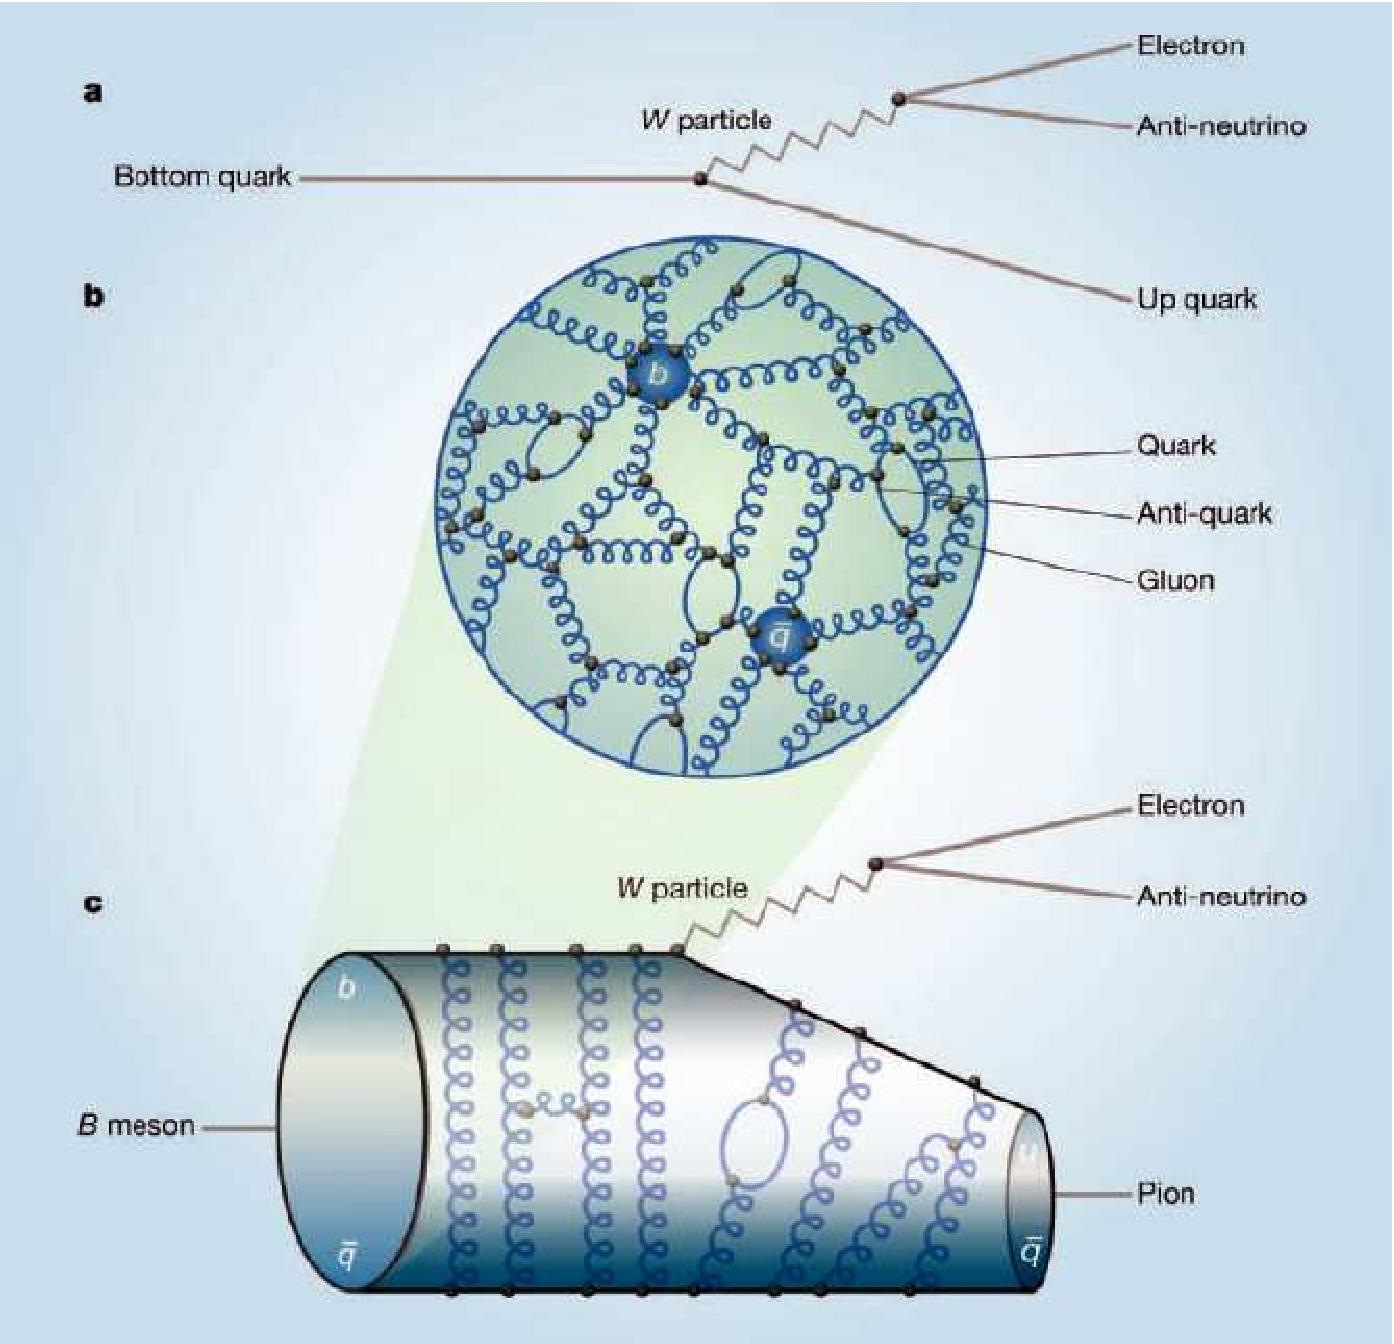
\includegraphics[width=0.7\linewidth]{ians_figure}
\end{center}
\vspace{-0.5 cm}

\end{slide}

%%%%%%%%%%%%%%%%%%%%%%%%%%%%%%%%%%%%%%%%%%%%%%%%%%%%%%%%%%%%%%%%%%%%%%%%%%%%%%

\begin{slide}
{\Huge \bf Outline for this Talk}

\vfill
\begin{center}
\begin{minipage}{0.8\linewidth} \Huge
\begin{enumerate}\setlength{\itemsep}{2 cm}

  \item Show how $V_{td}$ is obfuscated by QCD and how our knowledge
  of it is limited by our ability to compute QCD

  \item Introduce Lattice QCD as a tool which can help to compute the
  necessary parameter
  
  \item Describe a CLEO experiment which tests this calculation:
  di-electron widths of $\Upsilon(1S)$, $\Upsilon(2S)$, $\Upsilon(3S)$

\end{enumerate}
\end{minipage}
\end{center}
\vfill

\end{slide}

%%%%%%%%%%%%%%%%%%%%%%%%%%%%%%%%%%%%%%%%%%%%%%%%%%%%%%%%%%%%%%%%%%%%%%%%%%%%%%

\begin{slide}
{\Huge \bf Measuring $V_{td}$}

\vspace{0.75 cm}

\begin{tabular}{p{0.45\linewidth} p{0.45\linewidth}}
\begin{minipage}{\linewidth}
$B$-$\bar{B}$ mixing:

\vspace{0.25 cm}
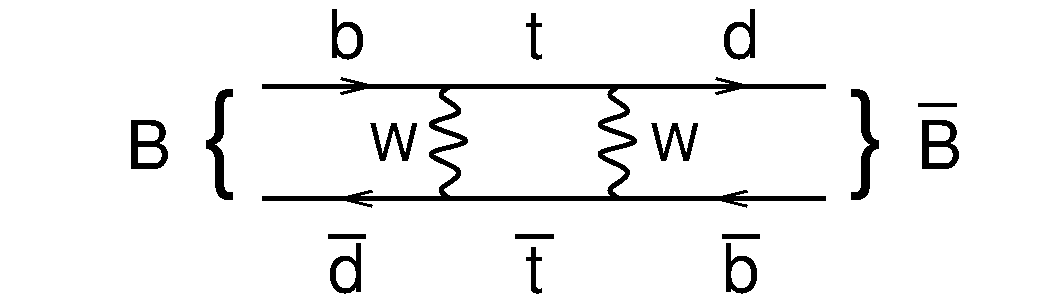
\includegraphics[width=\linewidth]{diagram_Bmix_box}

\end{minipage} &
\begin{minipage}{\linewidth}
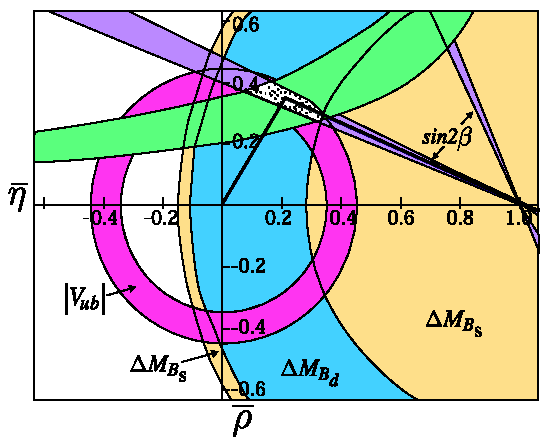
\includegraphics[width=\linewidth]{ckm04}
\end{minipage}
\end{tabular}

\vfill

$\Delta M_{B_d} = (known) \times ({f_B}^2 B_B) \times |V_{td}|^2$ = 0.510 $\pm$ 0.005 ps$^{-1}$, a 1\% measurement!

\vspace{1 cm}

But $f_B$ is only known to 20\% of itself

\vspace{1 cm}

Hence the 20\% uncertainty in $V_{td}$ (blue band)

\vfill
\end{slide}

%%%%%%%%%%%%%%%%%%%%%%%%%%%%%%%%%%%%%%%%%%%%%%%%%%%%%%%%%%%%%%%%%%%%%%%%%%%%%%

\begin{slide}
{\Huge \bf What is $f_B$?}

\vspace{0.75 cm}
QCD corrections to $b$-$\bar{d}$-electroweak ``vertex''

\vfill
\renewcommand{\arraystretch}{2}
\begin{tabular}{p{0.5\linewidth} p{0.4\linewidth}}
\begin{minipage}{\linewidth} On QCD length scales, B-mixing diagram \end{minipage} &
\begin{minipage}{\linewidth} looks like this: \end{minipage} \\
\begin{minipage}{\linewidth} 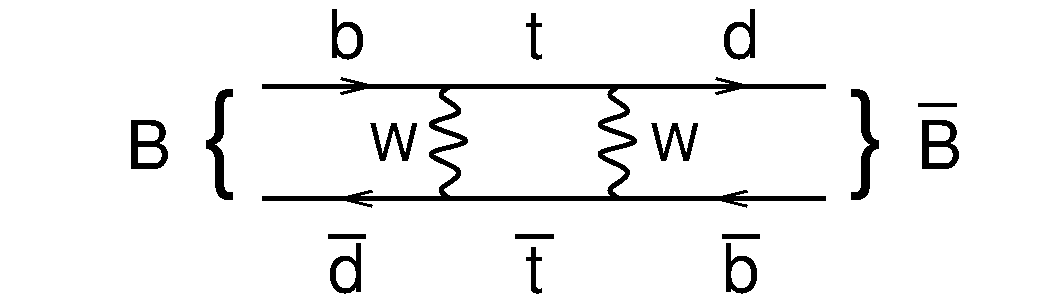
\includegraphics[width=12 cm]{diagram_Bmix_box} \end{minipage} &
\begin{minipage}{\linewidth} 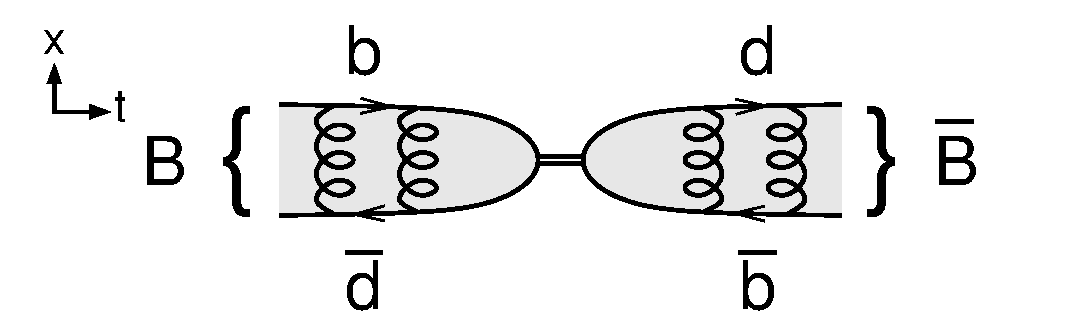
\includegraphics[width=12 cm]{diagram_Bmix} \end{minipage} \\
\end{tabular}

\vfill
\begin{tabular}{p{0.9\linewidth} p{0.05\linewidth}}
$f_B$ expresses the probability that the $\bar{d}$ will fluctuate onto the $b$ quark
\end{tabular}

\begin{tabular}{p{0.65\linewidth} p{0.23\linewidth}}
\begin{minipage}{\linewidth}

That is, the value of the spatial wavefunction at the origin

\end{minipage} &
\begin{minipage}{\linewidth}
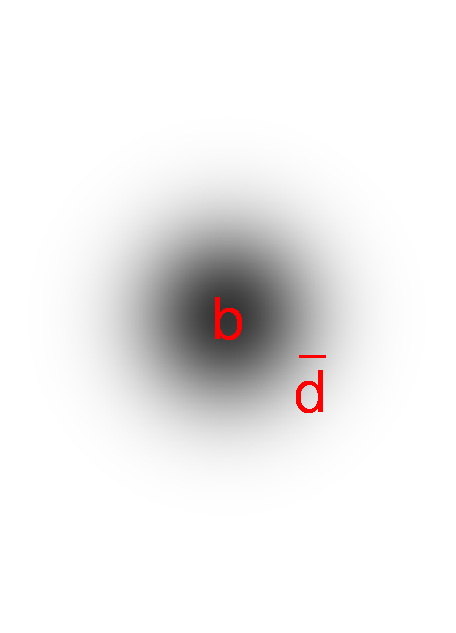
\includegraphics[width=\linewidth, trim=0 60 0 60, clip=true]{wavefunction_fb}
\end{minipage}
\end{tabular}

\vfill
\end{slide}

%%%%%%%%%%%%%%%%%%%%%%%%%%%%%%%%%%%%%%%%%%%%%%%%%%%%%%%%%%%%%%%%%%%%%%%%%%%%%%

\begin{slide}
{\Huge \bf Determining $f_B$}

\vspace{0.75 cm}
\begin{minipage}{0.5\linewidth} Experimentally? $B^- \to \ell^- \bar{\nu}$ \end{minipage} \hfill \begin{minipage}{12 cm} 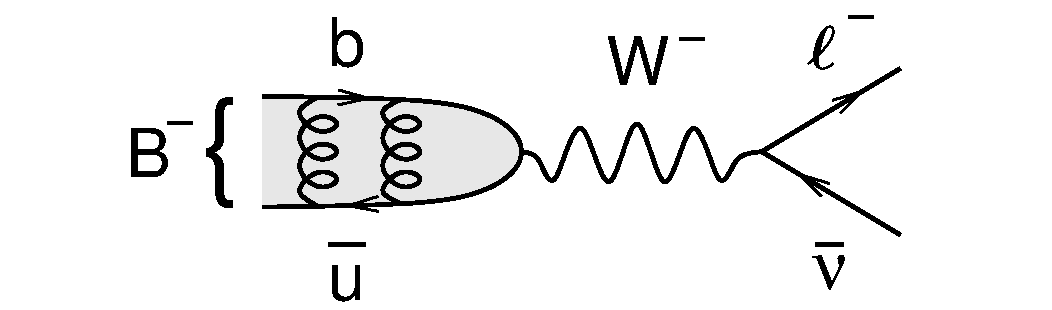
\includegraphics[width=\linewidth]{diagram_Btolnu} \end{minipage}

\begin{itemize}\setlength{\itemsep}{1.5 cm}

\newcommand{\mathheight}{{\color{white} \frac{\frac{\frac{!}{!}}{\frac{!}{!}}}{\frac{\frac{!}{!}}{!}}}}
\item $\displaystyle \Gamma(B^- \to \ell^- \bar{\nu}) = \frac{{G_F}^2}{8\pi} \ \underbrace{\mathheight |V_{ub}|^2 \mathheight}_{\mbox{small}} \ \underbrace{\mathheight {m_l}^2 M_B \left(1 - \frac{{m_l}^2}{{M_B}^2} \right)^2 \mathheight}_{\mbox{small}} \ {f_B}^2$

\item ${\cal B}(B^- \to \tau^- \bar{\nu}) <$ $\mathsf{1.8 \times 10^{-4}}$ at 90\% C.L. (253 fb$^{-1}$ at Belle 2005)
\end{itemize}

\vfill
\begin{minipage}{0.9\linewidth} Theoretically?  Need non-perturbative techniques\ldots \end{minipage}

\vfill
\end{slide}

%%%%%%%%%%%%%%%%%%%%%%%%%%%%%%%%%%%%%%%%%%%%%%%%%%%%%%%%%%%%%%%%%%%%%%%%%%%%%%

\begin{slide}
{\Huge \bf Lattice QCD}

\vspace{0.75 cm}
\begin{tabular}{p{0.65\linewidth} p{0.3\linewidth}}
\begin{minipage}{\linewidth}
\begin{itemize}

  \item Evaluate path integral with Monte Carlo integration

  \item Very computationally intensive

\end{itemize}
\end{minipage} &
\begin{minipage}{\linewidth}
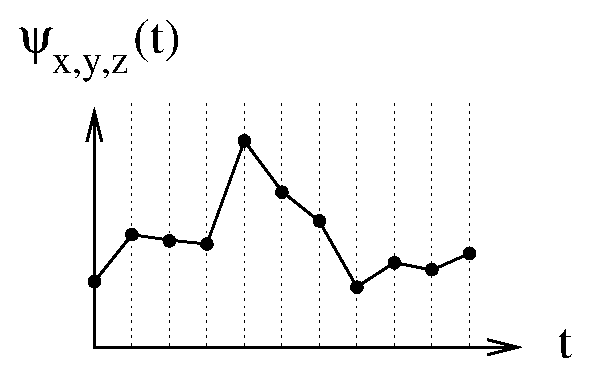
\includegraphics[width=\linewidth]{pathintegrals}
\end{minipage}
\end{tabular}

\vfill

\begin{center}
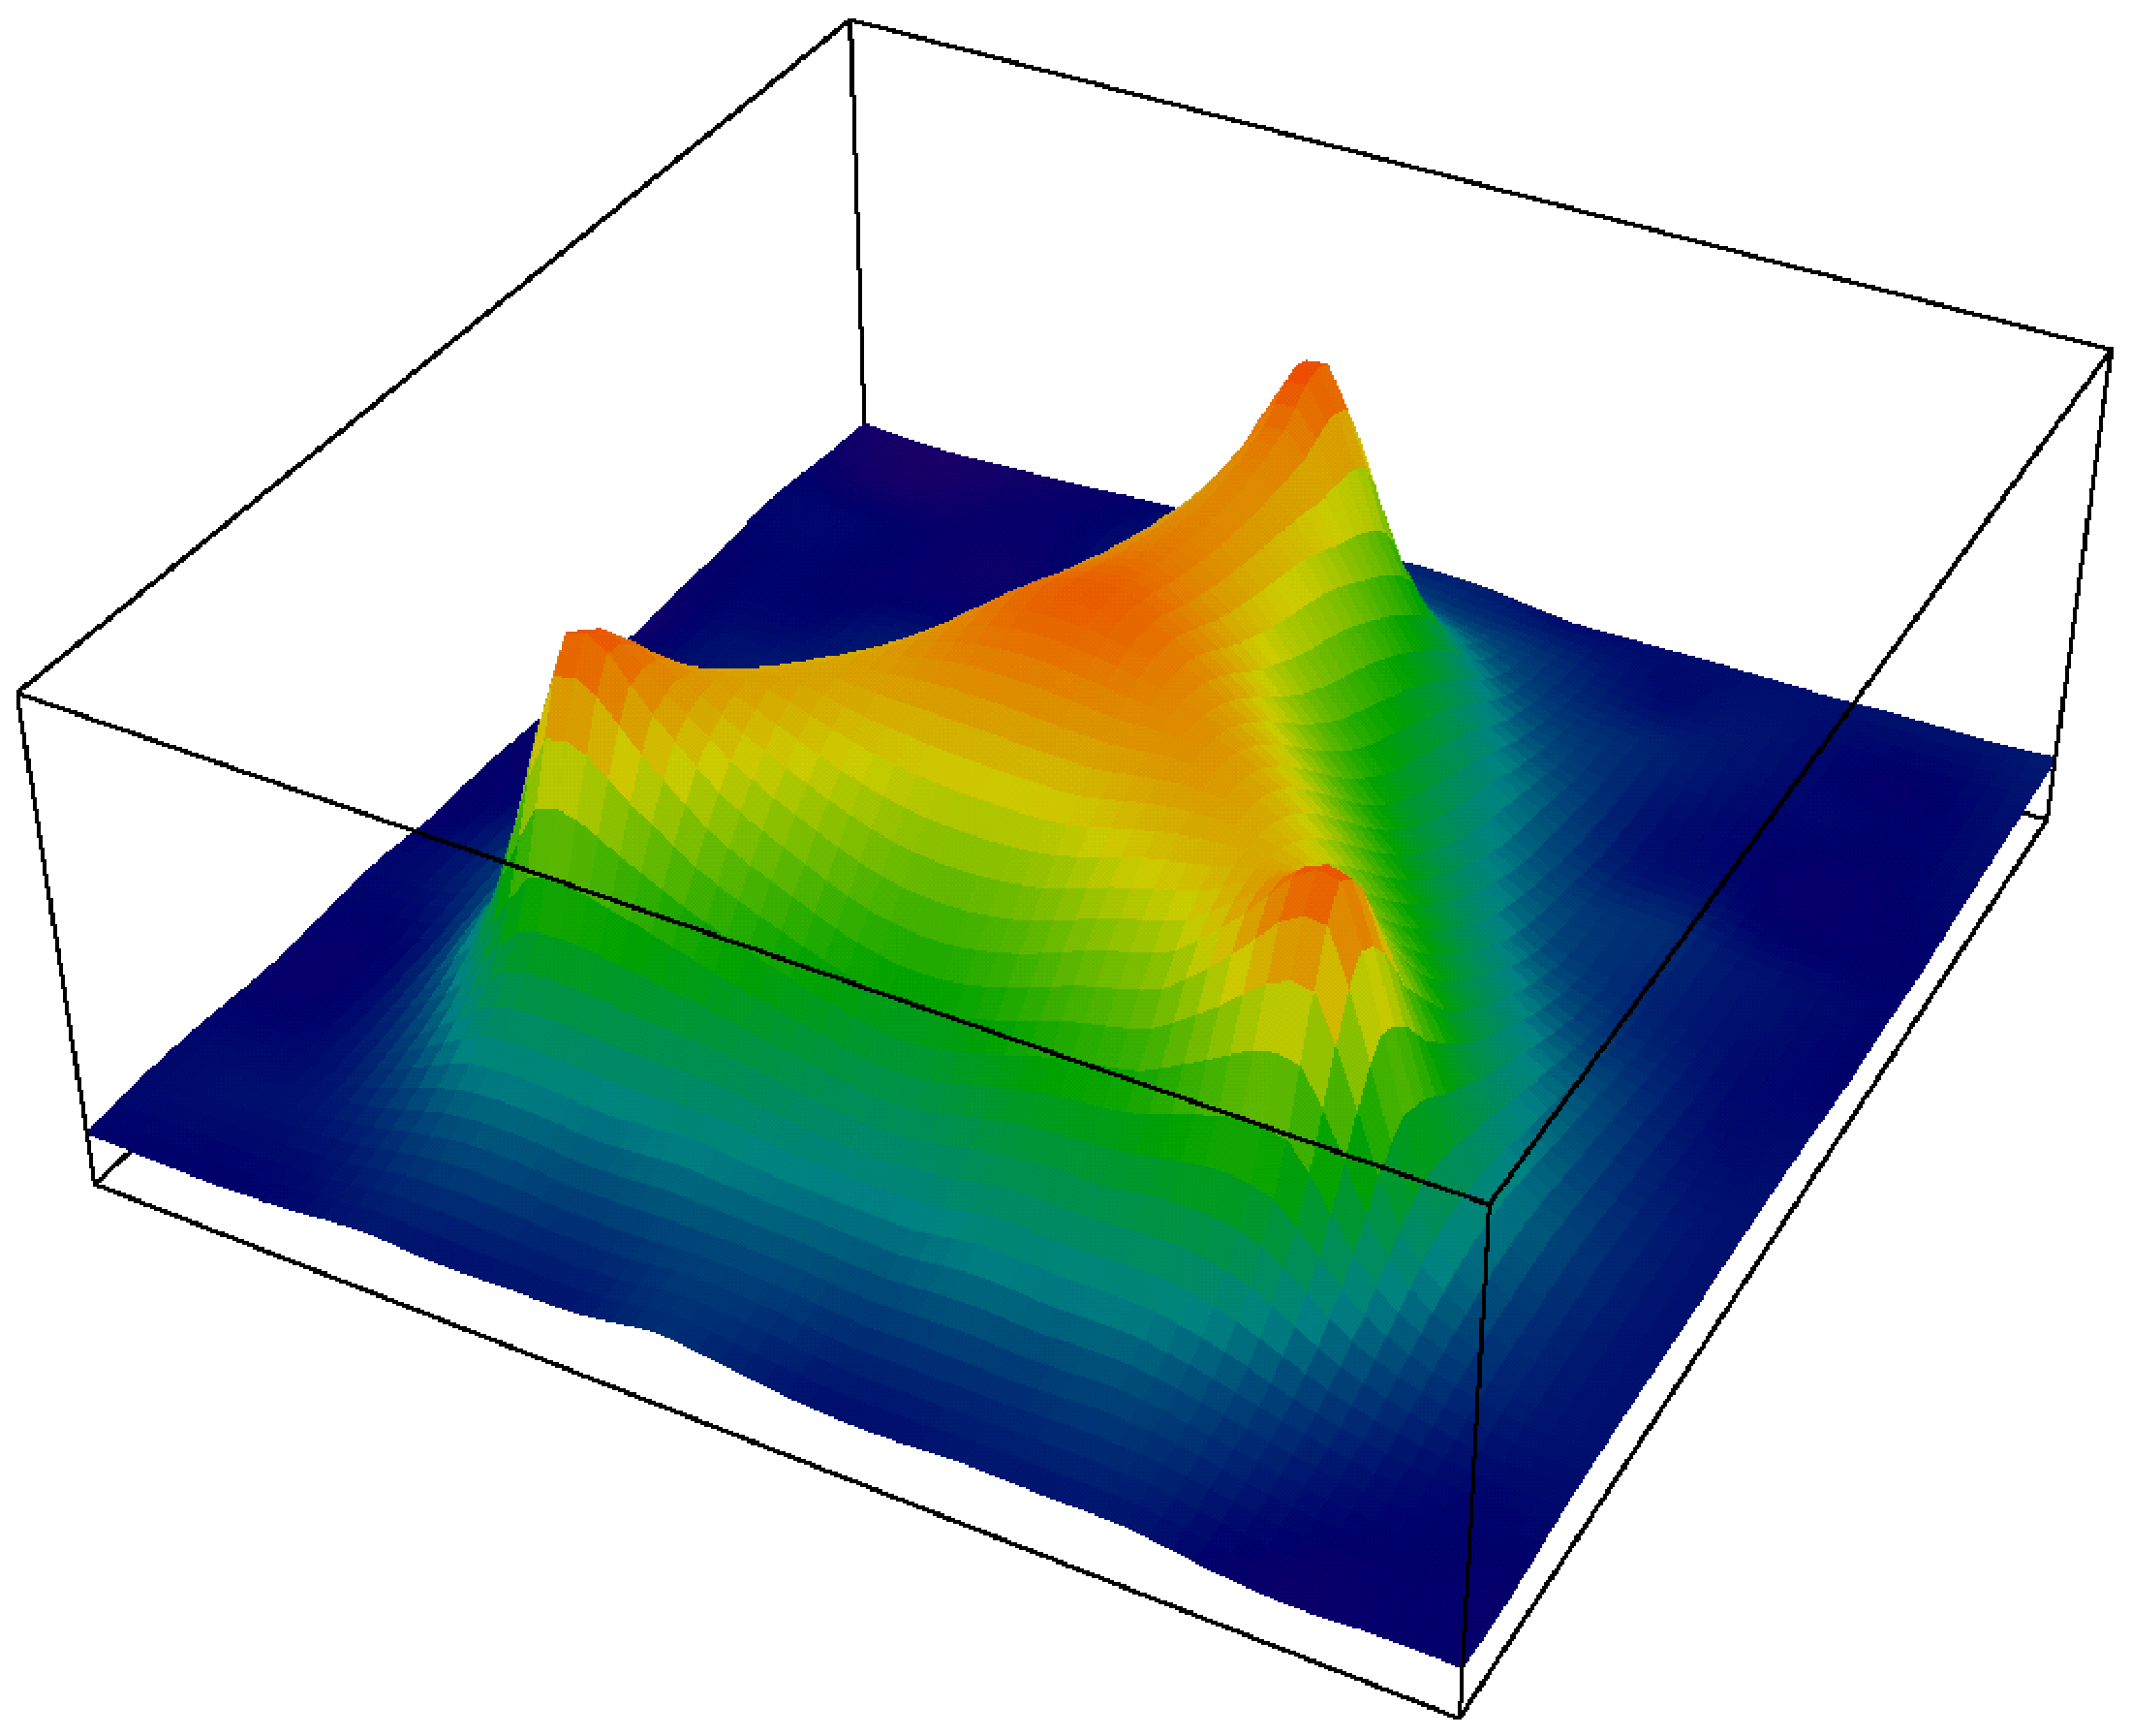
\includegraphics[width=0.5\linewidth]{qcd_proton}
\end{center}

\end{slide}

%%%%%%%%%%%%%%%%%%%%%%%%%%%%%%%%%%%%%%%%%%%%%%%%%%%%%%%%%%%%%%%%%%%%%%%%%%%%%%

\begin{slide}
{\Huge \bf Recent Breakthrough (c.\ 1999)}

\vfill
\begin{tabular}{p{0.5\linewidth} p{0.3\linewidth}}
\begin{minipage}{\linewidth}
Allows for calculation of vacuum polarization
\end{minipage} &
\begin{minipage}{\linewidth}
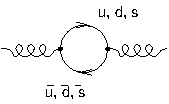
\includegraphics[height=3.5 cm]{vacuum_polarization}
\end{minipage}
\end{tabular}

\vfill
\begin{center}
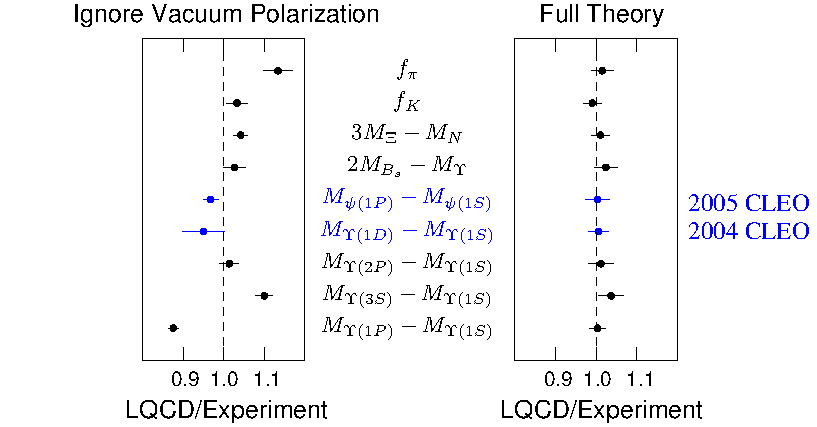
\includegraphics[width=0.85\linewidth]{lqcd_success}
\end{center}

\vfill
$\Omega^-$ and $B_c$ masses also confirmed to high accuracy
\end{slide}

%%%%%%%%%%%%%%%%%%%%%%%%%%%%%%%%%%%%%%%%%%%%%%%%%%%%%%%%%%%%%%%%%%%%%%%%%%%%%%

\begin{slide}
{\Huge \bf $f_B$ from Lattice QCD}

\vspace{0.75 cm}
$f_B = 216 \pm 9 \pm 19 \pm 4 \pm 6$ MeV \hfill Phys.\ Rev.\ Lett.\  {\bf 95}, 212001 (2005)

\vfill
\begin{center}
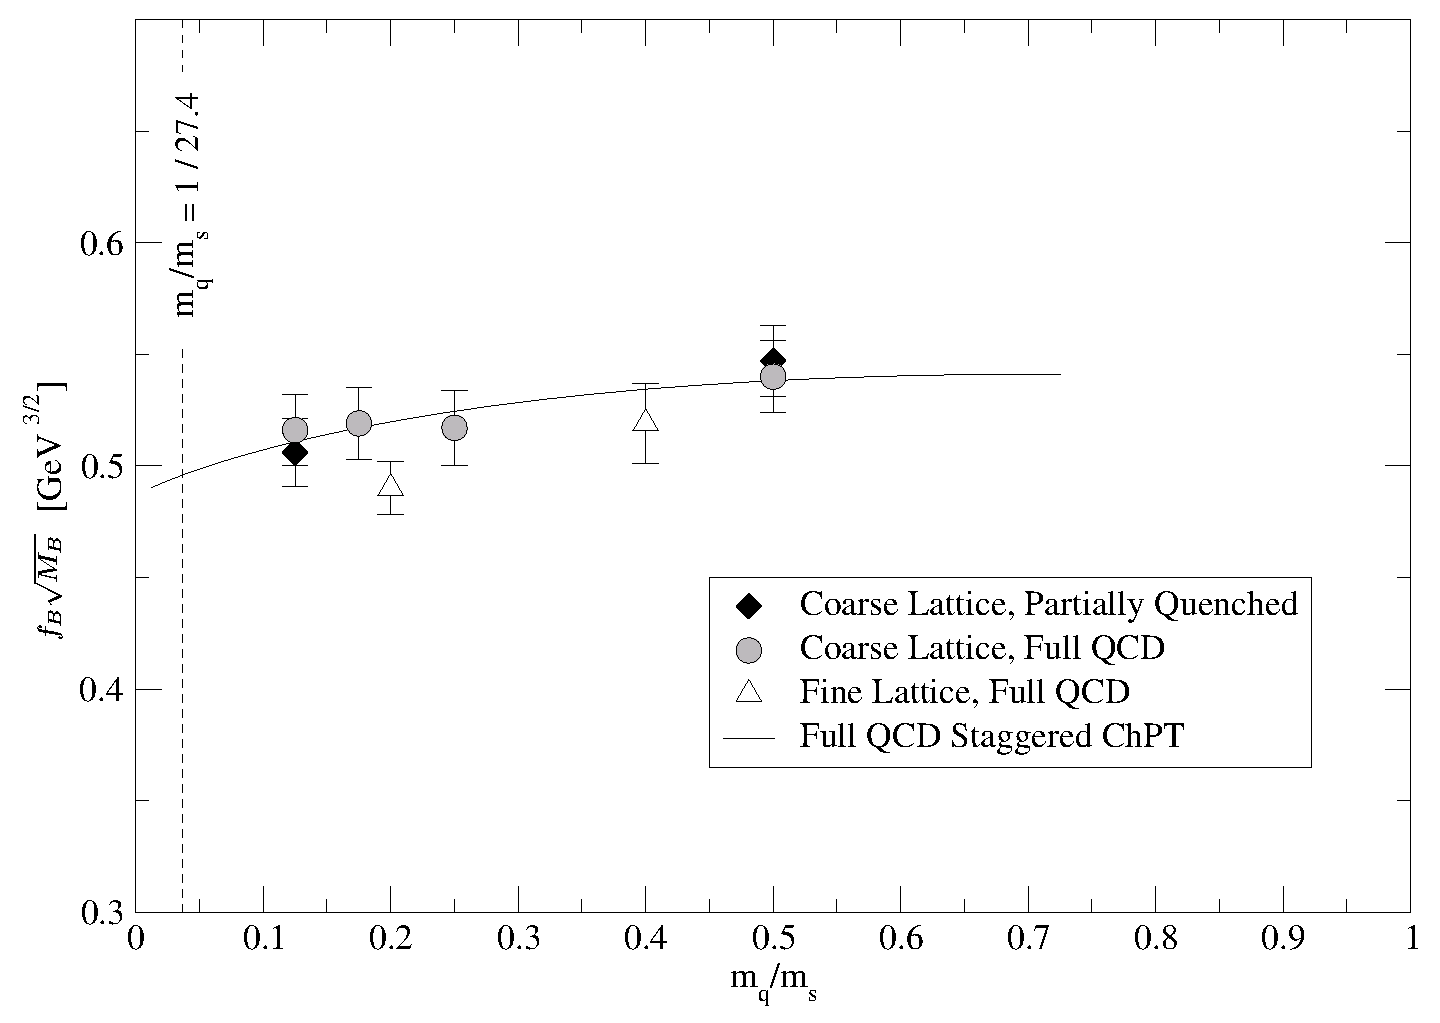
\includegraphics[width=0.7\linewidth]{fbresults}
\end{center}

\vfill
{\Huge \bf But how can we {\it verify} this?}

\vfill
\end{slide}

%%%%%%%%%%%%%%%%%%%%%%%%%%%%%%%%%%%%%%%%%%%%%%%%%%%%%%%%%%%%%%%%%%%%%%%%%%%%%%

\begin{slide}
{\Huge \bf Test with Processes that Differ by One Quark Flavor}

\vfill
\begin{minipage}{0.27\linewidth} \begin{center} {\Huge \boldmath $f_B$} \end{center} \end{minipage} \hfill \begin{minipage}{10 cm} 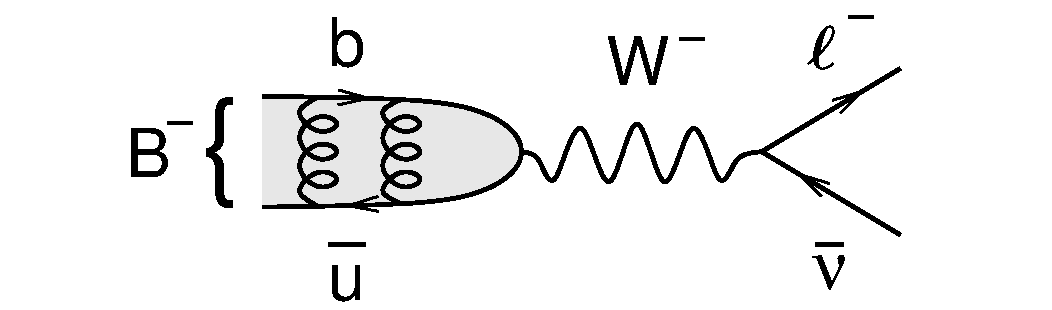
\includegraphics[width=\linewidth]{diagram_Btolnu} \end{minipage} \hfill \begin{minipage}{0.3\linewidth} \begin{center} LQCD only \end{center} \end{minipage}

\vfill
\begin{minipage}{0.27\linewidth} \begin{center} {\Huge \boldmath $f_D$} \end{center} \end{minipage} \hfill \begin{minipage}{10 cm} 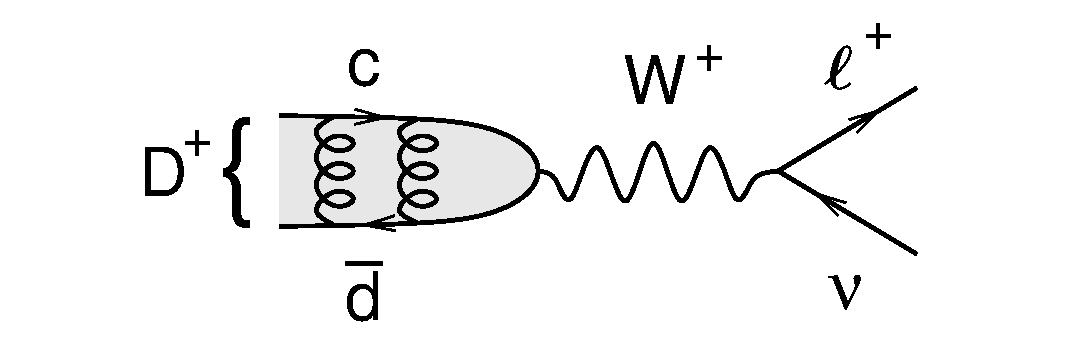
\includegraphics[width=\linewidth]{diagram_Dtolnu} \end{minipage} \hfill \begin{minipage}{0.3\linewidth} \begin{center} LQCD vs CLEO \end{center} \end{minipage}

\vfill
\fbox{\begin{minipage}{\linewidth}
\begin{minipage}{0.27\linewidth} \begin{center} {\Huge \boldmath $\Gamma(\Upsilon \to e^+e^-)$} \end{center} \end{minipage} \hfill \begin{minipage}{10 cm} 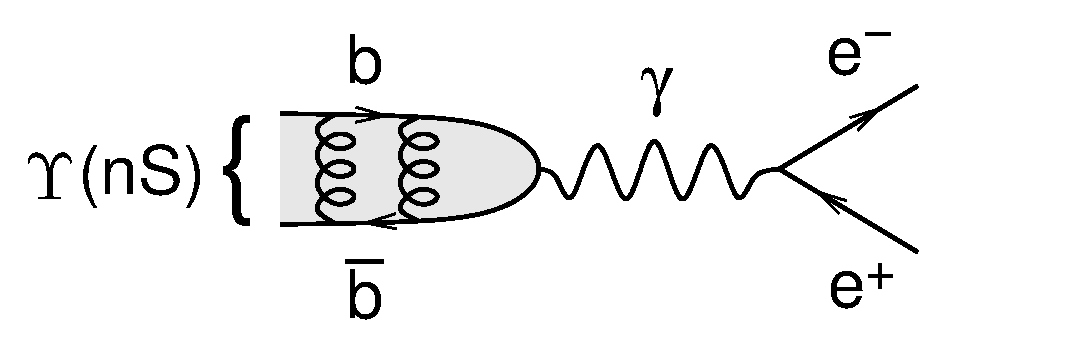
\includegraphics[width=\linewidth]{diagram_GeeU} \end{minipage} \hfill \begin{minipage}{0.3\linewidth} \begin{center} LQCD vs CLEO \end{center} \end{minipage}

\begin{minipage}{0.27\linewidth} \begin{center} ``Di-electron Width'' \end{center} \end{minipage}
\vspace{0.5 cm}
\end{minipage}}

\vfill
\end{slide}

%%%%%%%%%%%%%%%%%%%%%%%%%%%%%%%%%%%%%%%%%%%%%%%%%%%%%%%%%%%%%%%%%%%%%%%%%%%%%%

\begin{slide}
{\Huge \bf A Brief Look at $f_D$}

\vspace{0.75 cm}
CLEO-c: 281 pb$^{-1}$ at $\psi(3770)$ = 3 million $D^+D^-$ (30 times MARK-III, 8.5 times BES-II) % 9.6 pb-1, 33 pb-1

\vfill
\begin{center}
\begin{tabular}{p{0.45\linewidth} p{0.45\linewidth}}
\begin{minipage}{\linewidth}
\begin{center}
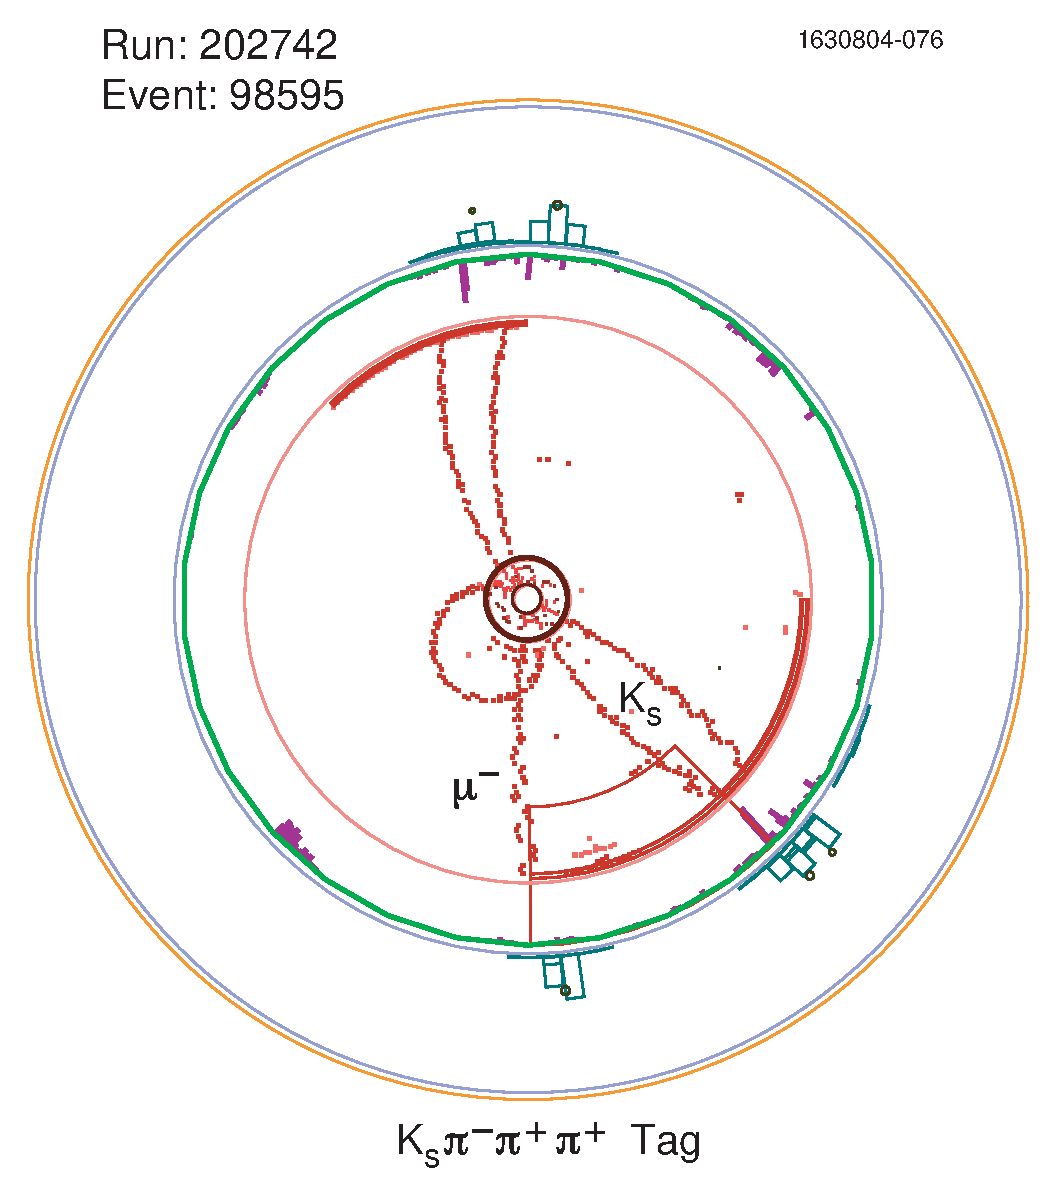
\includegraphics[width=0.8\linewidth]{dmunu_event}
\end{center}
\end{minipage} &
\begin{minipage}{\linewidth}
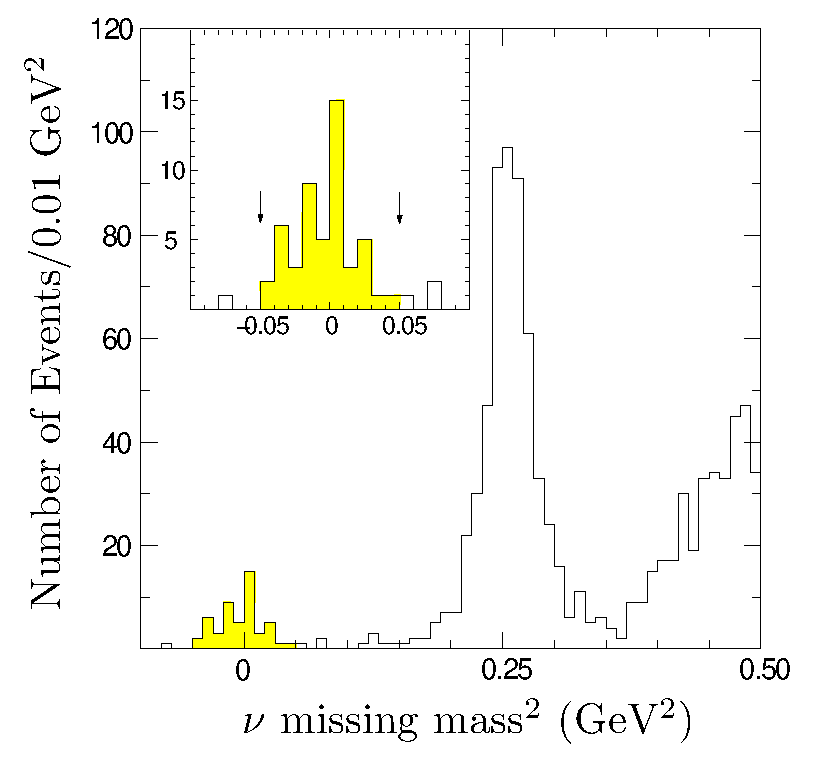
\includegraphics[width=\linewidth]{dmunu_mm}
\end{minipage}
\end{tabular}
\end{center}

\vfill
\mbox{\hspace{6.3 cm}} 50 events $-$ 2.8 background $=$ 47.2 $\pm$ 7.1 $^{\mathsf{+0.3}}_{\mathsf{-0.8}}$

\vfill
\mbox{\hspace{6.3 cm}} $\mathcal{B}(D^+ \to \mu^+\nu)$ = (4.40 $\pm$ 0.66 $^{{\mathsf{+0.09}}}_{{\mathsf{-0.12}}}$) $\times$ 10$^{{\mathsf{-4}}}$

\vfill
\mbox{\hspace{6.3 cm}} $f_{D^+}$ = (222.6 $\pm$ 16.7 $^{{\mathsf{+2.8}}}_{{\mathsf{-3.4}}}$) MeV

\vfill
\end{slide}

%%%%%%%%%%%%%%%%%%%%%%%%%%%%%%%%%%%%%%%%%%%%%%%%%%%%%%%%%%%%%%%%%%%%%%%%%%%%%%

\begin{slide}
{\Huge \bf A Brief Look at $f_D$}

\vspace{0.75 cm}
\begin{center}
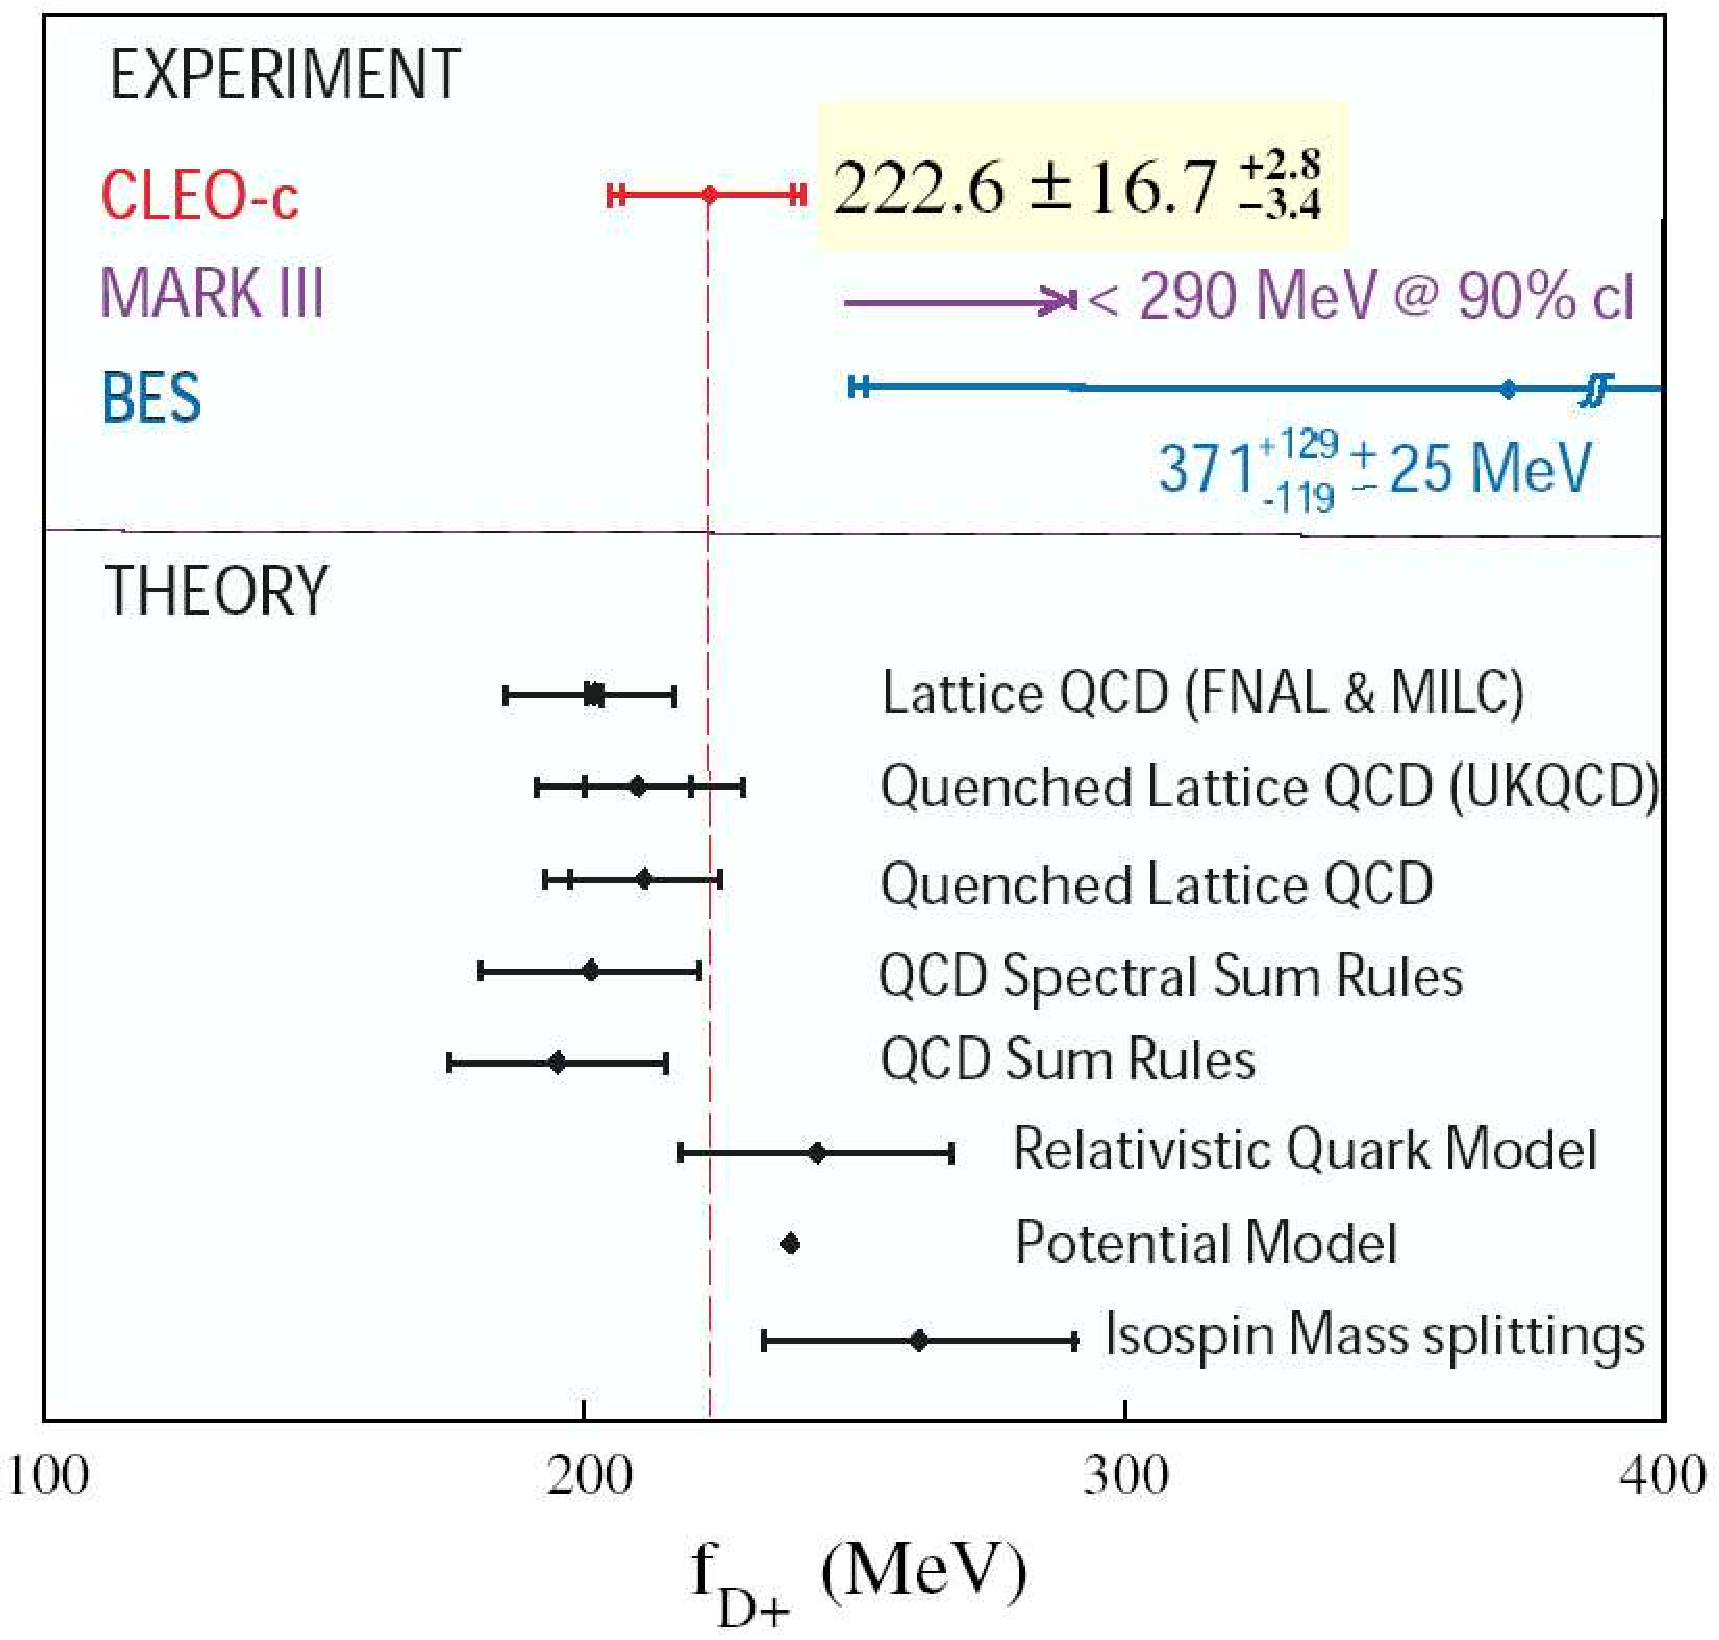
\includegraphics[width=0.55\linewidth]{dmunu_comparison3}
\end{center}

\vfill
Projected final precision: 4.5\% on $f_D$ and 4.5\% on $f_{D_s}$

\vfill
{\Large M.~Artuso {\it et al.} (CLEO Collaboration) Phys.\ Rev.\ Lett.\ {\bf 95}, 251801 (2005)}
\end{slide}

%%%%%%%%%%%%%%%%%%%%%%%%%%%%%%%%%%%%%%%%%%%%%%%%%%%%%%%%%%%%%%%%%%%%%%%%%%%%%%

\begin{slidemap}[technique & efficiency & backgrounds & luminosity & energy & fits & results & theory]
\mbox{ }
\vfill
\begin{center}
{\Huge \bf \boldmath Di-electron widths of $\Upsilon(1S)$, $\Upsilon(2S)$, $\Upsilon(3S)$}

\vspace{1 cm}
\begin{minipage}{0.7\linewidth}
\begin{itemize}\setlength{\itemsep}{0.5 cm}

\item Three high-precision measurements (1.5\%, 1.8\%, and 1.8\%)

\item Largely share systematics

\item See top of screen for an outline

\end{itemize}
\end{minipage}
\end{center}
\vfill
\mbox{ }
\end{slidemap}

%%%%%%%%%%%%%%%%%%%%%%%%%%%%%%%%%%%%%%%%%%%%%%%%%%%%%%%%%%%%%%%%%%%%%%%%%%%%%%

\begin{slidemap}[\textcolor{blue}{technique} & efficiency & backgrounds & luminosity & energy & fits & results & theory]
Di-electron width $\Gamma_{ee}$ = rate of $\Upsilon \to e^+e^-$ = $\Gamma \times {\mathcal B}_{ee}$

\vfill
Cannot obtain $\Gamma_{ee}$ from ${\mathcal B}_{ee}$ because $\Gamma$ is unresolvable

\vfill
\begin{tabular}{p{5.3 cm} p{8 cm} p{1 cm} p{8 cm}}
\begin{minipage}{\linewidth} \hspace{-0.4 cm} Instead, determine \end{minipage} &
\begin{minipage}{\linewidth} 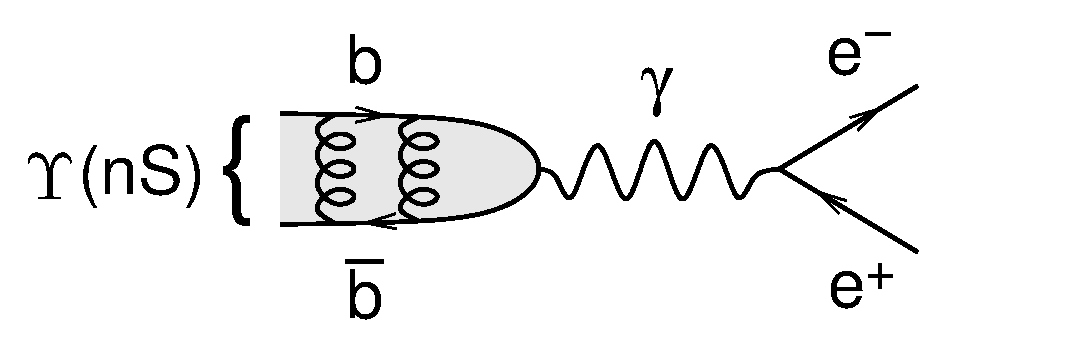
\includegraphics[width=\linewidth, trim=0 0 50 0]{diagram_GeeU} \end{minipage} &
\begin{minipage}{\linewidth} from \end{minipage} &
\begin{minipage}{\linewidth} 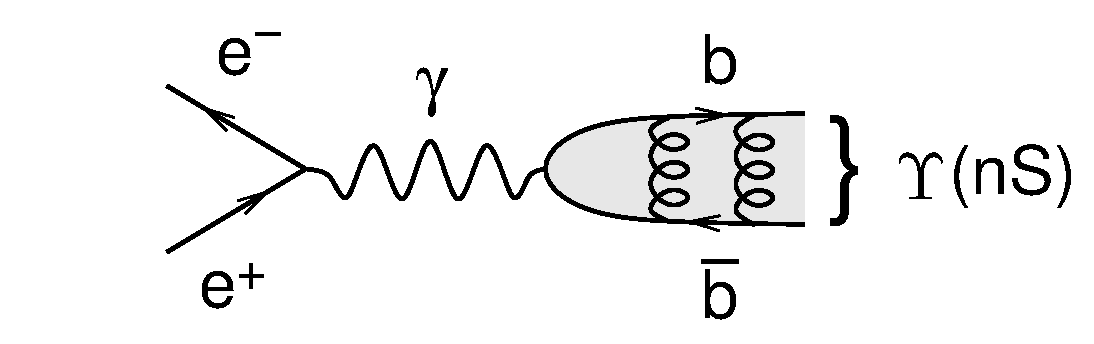
\includegraphics[width=\linewidth, trim=40 0 40 0]{diagram_GeeU-reversed} \end{minipage}
\end{tabular}

\vfill
\begin{center}
\includegraphics[width=0.5\linewidth]{equation}\end{center}

\vfill
Scan $e^+e^-$ collision energies across $M_\Upsilon$, measure cross-section $\sigma(E)$, and integrate

\vfill
\end{slidemap}

%%%%%%%%%%%%%%%%%%%%%%%%%%%%%%%%%%%%%%%%%%%%%%%%%%%%%%%%%%%%%%%%%%%%%%%%%%%%%%

\begin{slidemap}[\textcolor{blue}{technique} & efficiency & backgrounds & luminosity & energy & fits & results & theory]

\vspace{-1 cm}
\begin{center}
\includegraphics[width=0.5\linewidth]{equation}\end{center}

\begin{center}
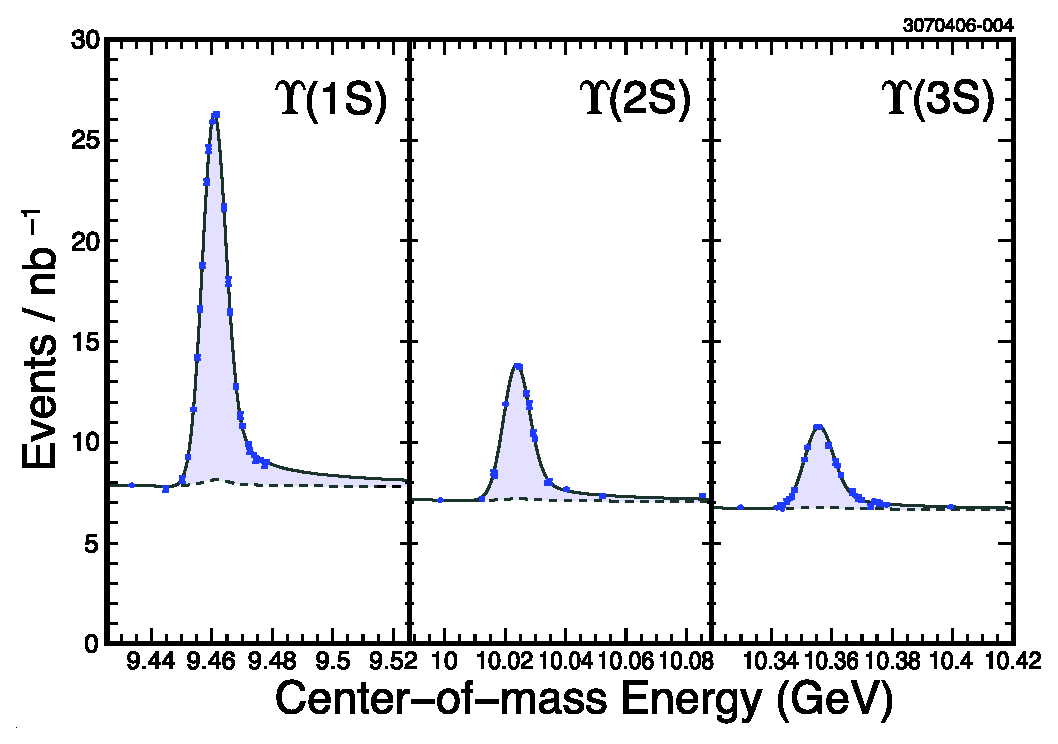
\includegraphics[width=0.7\linewidth]{peaks}
\end{center}

\vfill
10\% of CLEO's $\Upsilon(1S)$, $\Upsilon(2S)$, $\Upsilon(3S)$ program
\end{slidemap}

%%%%%%%%%%%%%%%%%%%%%%%%%%%%%%%%%%%%%%%%%%%%%%%%%%%%%%%%%%%%%%%%%%%%%%%%%%%%%%

\begin{slidemap}[\textcolor{blue}{technique} & efficiency & backgrounds & luminosity & energy & fits & results & theory]
{\Huge \bf Anatomy of an $\Upsilon$ Lineshape}

\vspace{0.75 cm}
\begin{center}
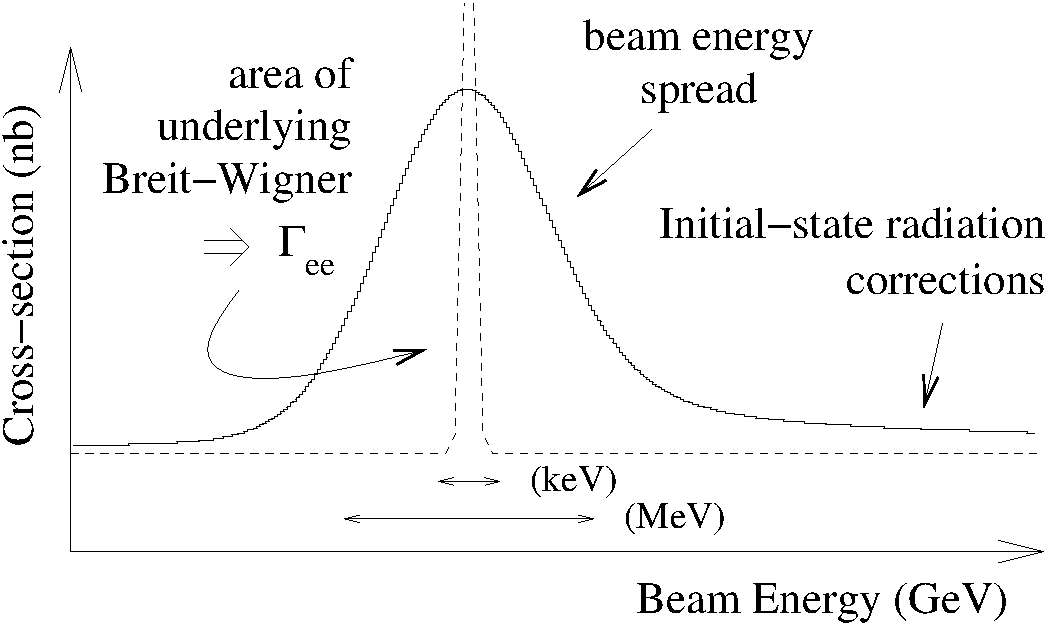
\includegraphics[width=0.6\linewidth]{cartoon}
\end{center}

\begin{itemize}

  \item Breit-Wigner resonance is convoluted by beam energy spread

  \item Further spread by initial-state radiation ($e^+e^- \to \gamma \Upsilon$)
  
  \item Flat backgrounds

\end{itemize}

Simulate all effects with a fit function, report Breit-Wigner area only

\vfill
\end{slidemap}

%%%%%%%%%%%%%%%%%%%%%%%%%%%%%%%%%%%%%%%%%%%%%%%%%%%%%%%%%%%%%%%%%%%%%%%%%%%%%%

\begin{slidemap}[\textcolor{blue}{technique} & efficiency & backgrounds & luminosity & energy & fits & results & theory]
\begin{center}
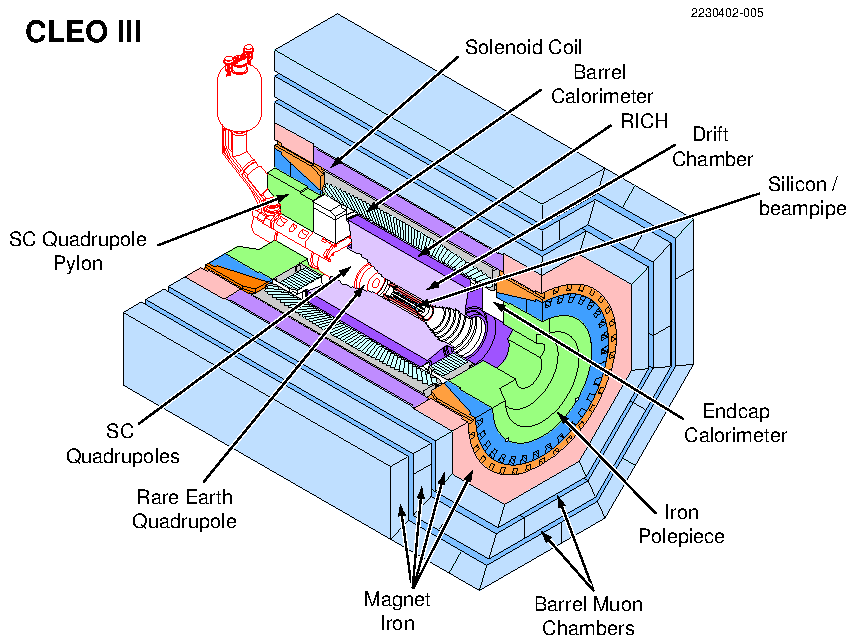
\includegraphics[width=0.75\linewidth]{cleo3}
\end{center}
\vfill
\end{slidemap}

%%%%%%%%%%%%%%%%%%%%%%%%%%%%%%%%%%%%%%%%%%%%%%%%%%%%%%%%%%%%%%%%%%%%%%%%%%%%%%

\begin{slidemap}[\textcolor{blue}{technique} & efficiency & backgrounds & luminosity & energy & fits & results & theory]
{\Huge \bf Event Selection}

\vspace{0.75 cm}
\begin{center}
  \begin{tabular}{p{0.6\linewidth} p{0.3\linewidth}}
    \begin{minipage}{\linewidth}
      \begin{center}
	\LARGE Solid = data, dashed = scaled Monte Carlo, log scale

	\vspace{0.5 cm}
	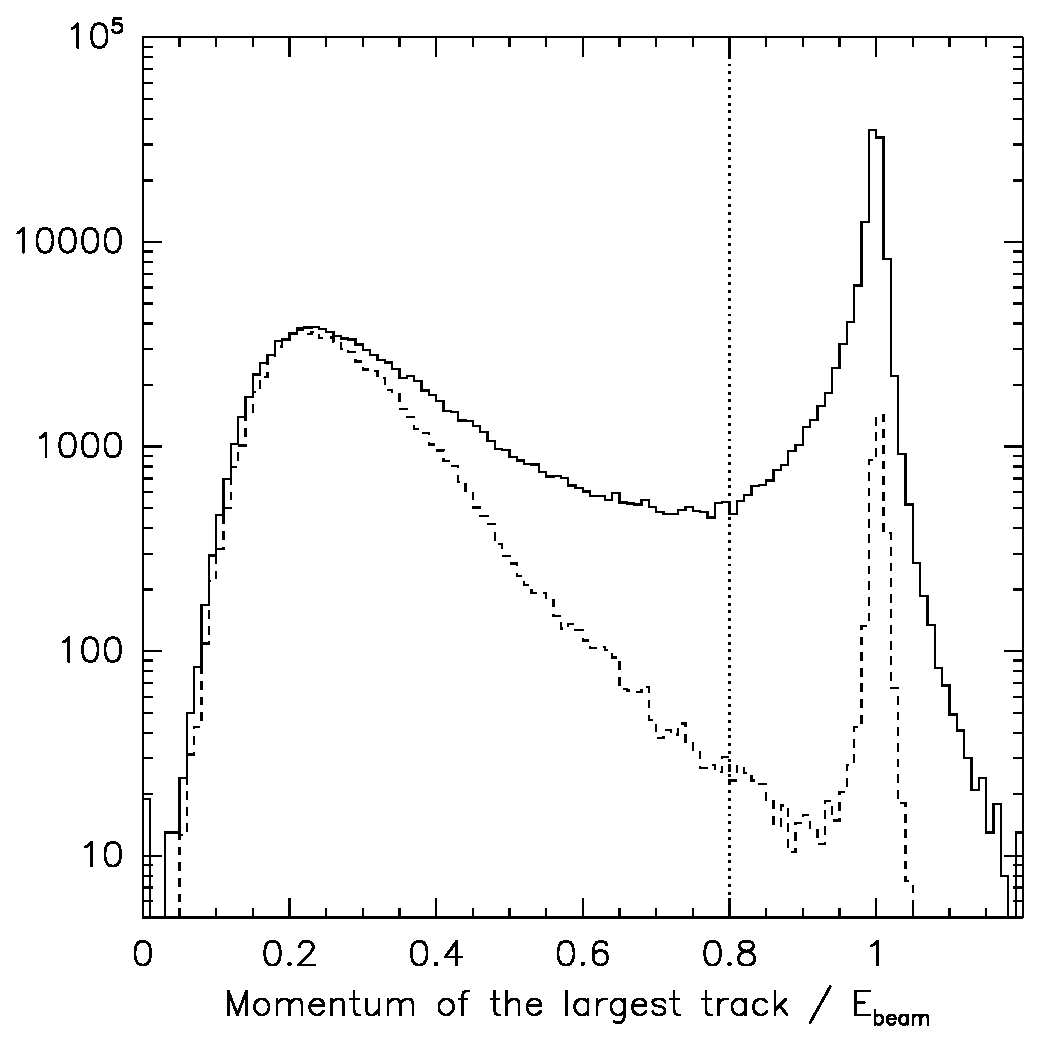
\includegraphics[width=0.8\linewidth, height=0.8\linewidth]{cuts_p1} \mbox{\hspace{1 cm}}
      \end{center}
    \end{minipage} & 
    \begin{minipage}{\linewidth}
      Rejects

      \vspace{0.5 cm}
      \begin{enumerate}\setlength{\itemsep}{1 cm}

	\item \textcolor{blue}{Bhabhas}

	\item \textcolor{white}{Two-photon fusion}

	\item \textcolor{white}{Cosmic rays}

	\item \textcolor{white}{Beam-gas}

      \end{enumerate}
    \end{minipage}
  \end{tabular}
\end{center}

\vfill
\end{slidemap}

%%%%%%%%%%%%%%%%%%%%%%%%%%%%%%%%%%%%%%%%%%%%%%%%%%%%%%%%%%%%%%%%%%%%%%%%%%%%%%

\begin{slidemap}[\textcolor{blue}{technique} & efficiency & backgrounds & luminosity & energy & fits & results & theory]
{\Huge \bf Event Selection}

\vspace{0.75 cm}
\begin{center}
  \begin{tabular}{p{0.6\linewidth} p{0.3\linewidth}}
    \begin{minipage}{\linewidth}
      \begin{center}
	\LARGE Solid = data, dashed = scaled Monte Carlo, log scale

	\vspace{0.5 cm}
	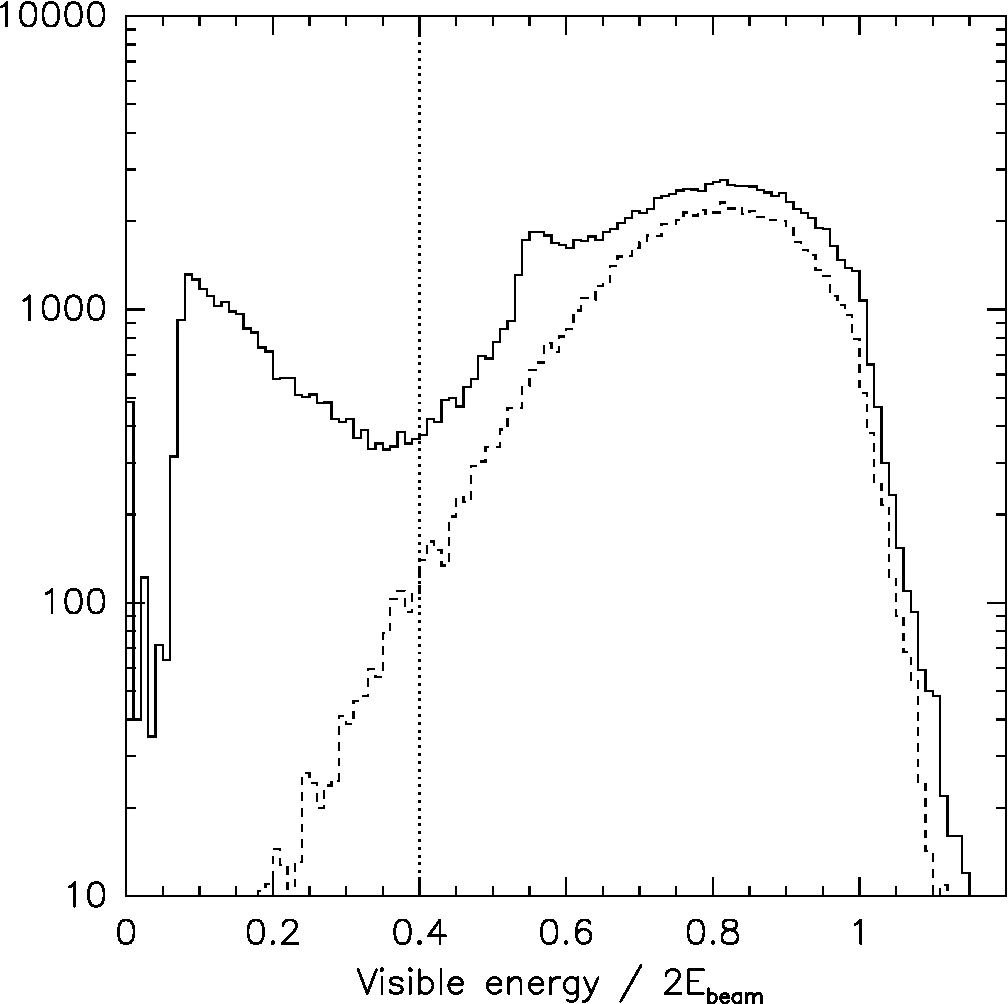
\includegraphics[width=0.8\linewidth, height=0.8\linewidth]{cuts_visen} \mbox{\hspace{1 cm}}
      \end{center}
    \end{minipage} & 
    \begin{minipage}{\linewidth}
      Rejects

      \vspace{0.5 cm}
      \begin{enumerate}\setlength{\itemsep}{1 cm}

	\item \textcolor{black}{Bhabhas}

	\item \textcolor{blue}{Two-photon fusion}

	\item \textcolor{white}{Cosmic rays}

	\item \textcolor{white}{Beam-gas}

      \end{enumerate}
    \end{minipage}
  \end{tabular}
\end{center}

\vfill
\end{slidemap}

%%%%%%%%%%%%%%%%%%%%%%%%%%%%%%%%%%%%%%%%%%%%%%%%%%%%%%%%%%%%%%%%%%%%%%%%%%%%%%

\begin{slidemap}[\textcolor{blue}{technique} & efficiency & backgrounds & luminosity & energy & fits & results & theory]
{\Huge \bf Event Selection}

\vspace{0.75 cm}
\begin{center}
  \begin{tabular}{p{0.6\linewidth} p{0.3\linewidth}}
    \begin{minipage}{\linewidth}
      \begin{center}
	\LARGE Solid = data, dashed = scaled Monte Carlo, log scale

	\vspace{0.5 cm}
	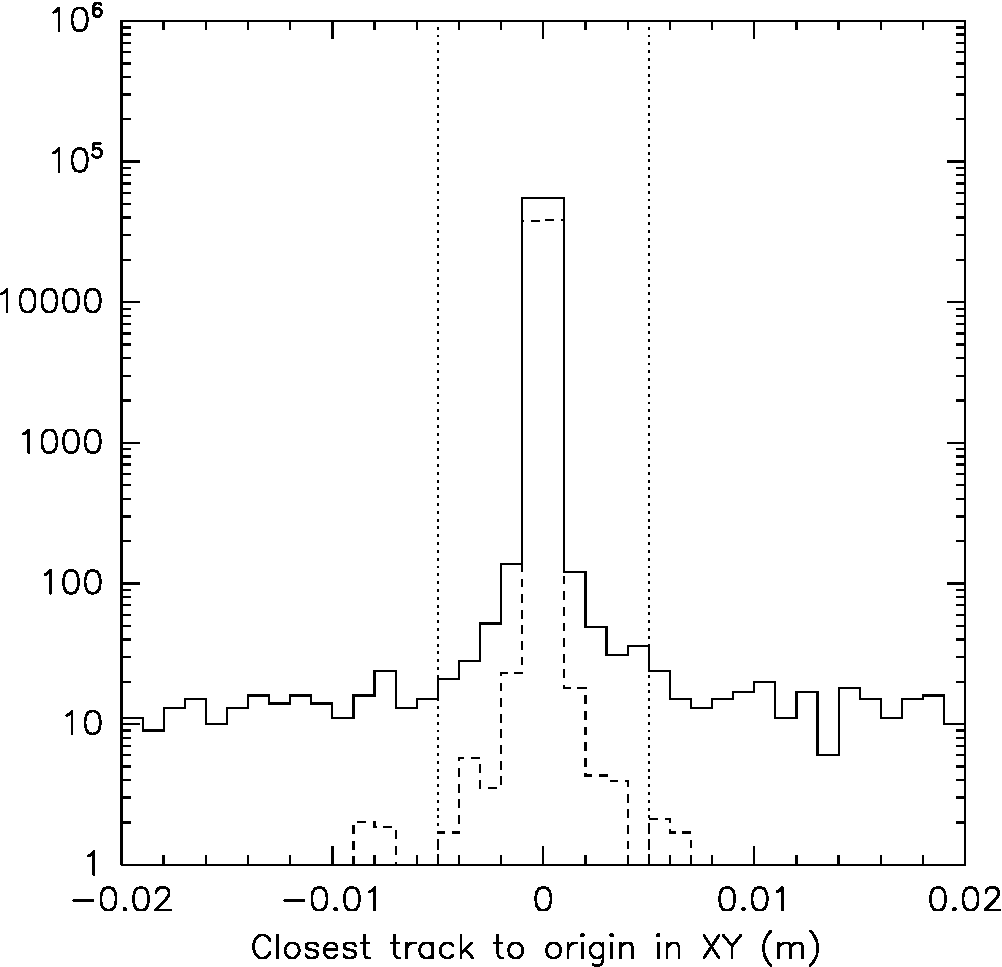
\includegraphics[width=0.8\linewidth, height=0.8\linewidth]{cuts_d0close} \mbox{\hspace{1 cm}}
      \end{center}
    \end{minipage} & 
    \begin{minipage}{\linewidth}
      Rejects

      \vspace{0.5 cm}
      \begin{enumerate}\setlength{\itemsep}{1 cm}

	\item \textcolor{black}{Bhabhas}

	\item \textcolor{black}{Two-photon fusion}

	\item \textcolor{blue}{Cosmic rays}

	\item \textcolor{white}{Beam-gas}

      \end{enumerate}
    \end{minipage}
  \end{tabular}
\end{center}

\vfill
\end{slidemap}

%%%%%%%%%%%%%%%%%%%%%%%%%%%%%%%%%%%%%%%%%%%%%%%%%%%%%%%%%%%%%%%%%%%%%%%%%%%%%%

\begin{slidemap}[\textcolor{blue}{technique} & efficiency & backgrounds & luminosity & energy & fits & results & theory]
{\Huge \bf Event Selection}

\vspace{0.75 cm}
\begin{center}
  \begin{tabular}{p{0.6\linewidth} p{0.3\linewidth}}
    \begin{minipage}{\linewidth}
      \begin{center}
	\LARGE Solid = data, dashed = scaled Monte Carlo, log scale

	\vspace{0.5 cm}
	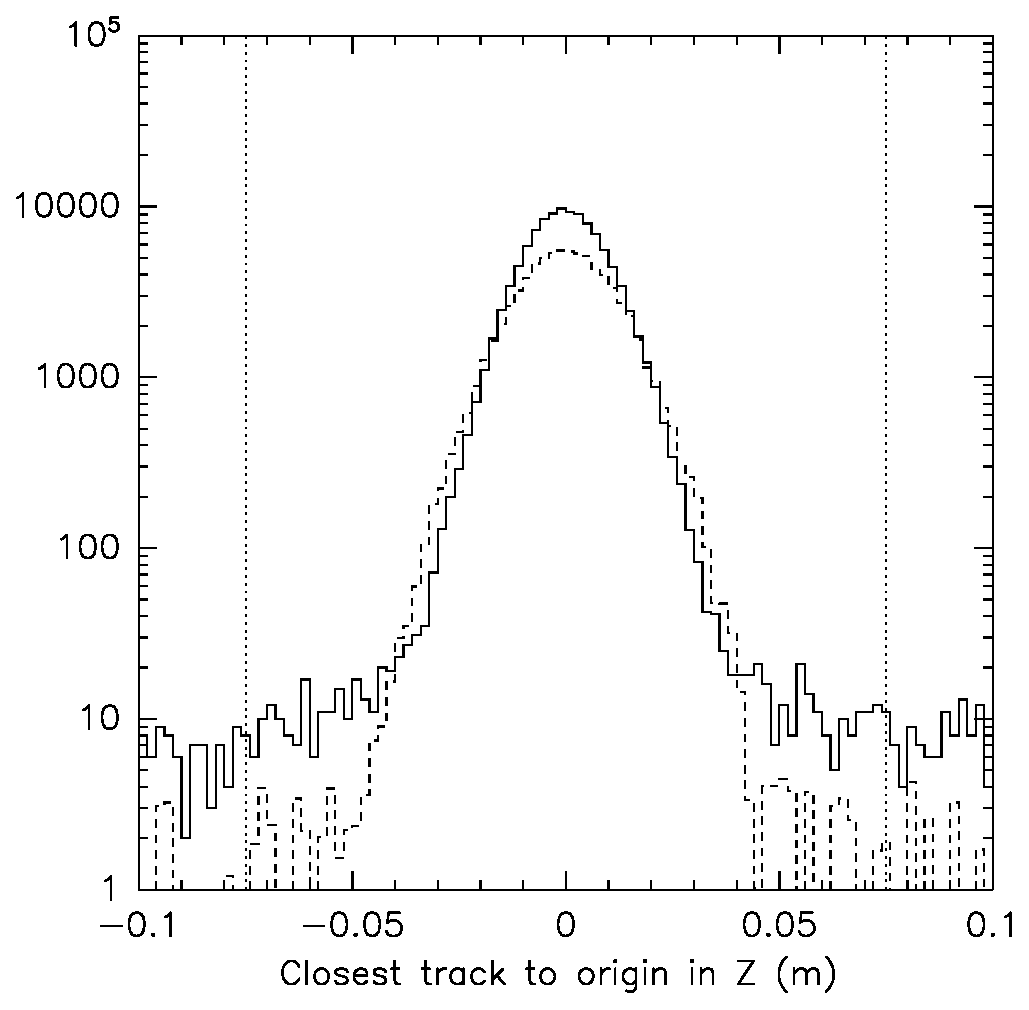
\includegraphics[width=0.8\linewidth, height=0.8\linewidth]{cuts_anyz} \mbox{\hspace{1 cm}}
      \end{center}
    \end{minipage} & 
    \begin{minipage}{\linewidth}
      Rejects

      \vspace{0.5 cm}
      \begin{enumerate}\setlength{\itemsep}{1 cm}

	\item \textcolor{black}{Bhabhas}

	\item \textcolor{black}{Two-photon fusion}

	\item \textcolor{black}{Cosmic rays}

	\item \textcolor{blue}{Beam-gas}

      \end{enumerate}
    \end{minipage}
  \end{tabular}
\end{center}

\vfill
\end{slidemap}

%%%%%%%%%%%%%%%%%%%%%%%%%%%%%%%%%%%%%%%%%%%%%%%%%%%%%%%%%%%%%%%%%%%%%%%%%%%%%%

\begin{slidemap}[technique & \textcolor{blue}{efficiency} & backgrounds & luminosity & energy & fits & results & theory]
Event selection rejects $e^+e^-$, $\mu^+\mu^-$, and 43\% of $\tau^+\tau^-$

\vfill
Correct apparent cross-section with $\displaystyle \frac{1}{1 - 2.43{\mathcal B}_{\mu\mu}}$

\vfill
Define hadronic efficiency = probability that non-leptonic decays pass cuts and trigger

\vfill
{\Huge \bf Data-Derived Efficiency Study}

\begin{itemize}

  \item Select $\Upsilon(2S) \to \pi^+\pi^- \Upsilon(1S)$ events by the $\pi^+\pi^-$ only

  \item Count how many $\Upsilon(1S)$ decays pass cuts and trigger

\end{itemize}

\begin{center}
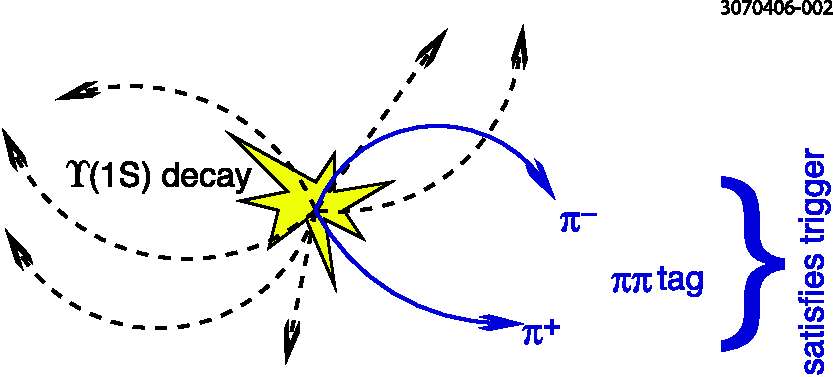
\includegraphics[width=0.5\linewidth]{efficiency_cartoon}
\end{center}

Includes as-yet unknown decay modes
\end{slidemap}

%%%%%%%%%%%%%%%%%%%%%%%%%%%%%%%%%%%%%%%%%%%%%%%%%%%%%%%%%%%%%%%%%%%%%%%%%%%%%%

\begin{slidemap}[technique & \textcolor{blue}{efficiency} & backgrounds & luminosity & energy & fits & results & theory]
{\Huge \bf Data-Derived Efficiency Study}

\begin{itemize}

  \item Select $\Upsilon(2S) \to \pi^+\pi^- \Upsilon(1S)$ events by the $\pi^+\pi^-$ only

  \item Count how many $\Upsilon(1S)$ decays pass cuts and trigger

\end{itemize}

\begin{center}
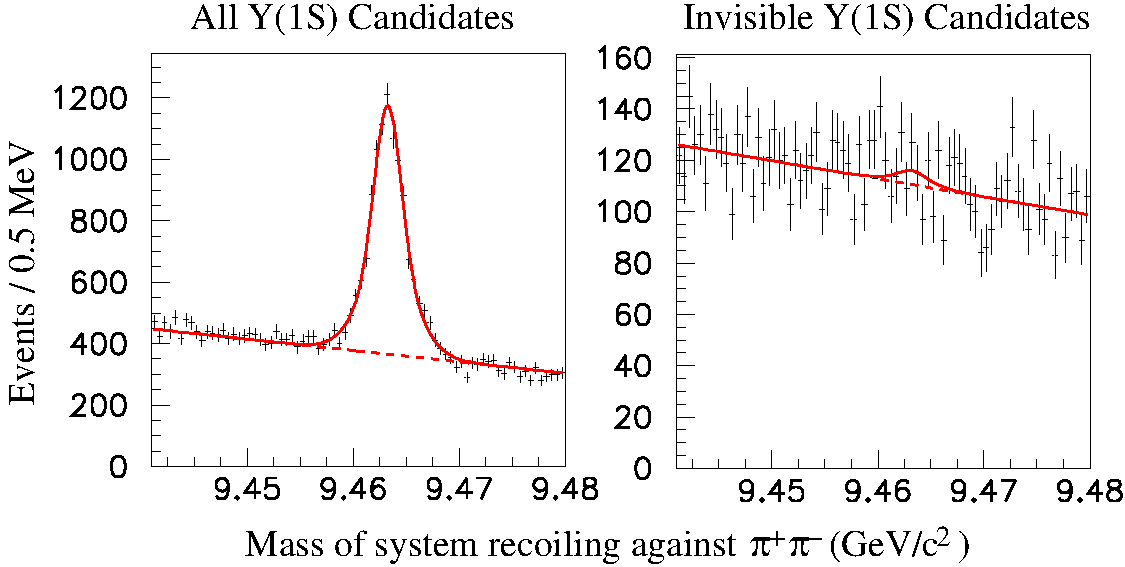
\includegraphics[width=0.7\linewidth]{efficiency_recoilmasses}
\end{center}

\begin{itemize}

  \item $\Upsilon(1S)$ hadronic efficiency is 97.8\% $\pm$ 0.5\%

  \item 90\% upper limit on invisible $\Upsilon(1S)$ decays is ${\mathcal B}_{\mbox{\Large inv}} <$ 1.0\% 

\end{itemize}

\vfill
For $\Upsilon(2S)$ and $\Upsilon(3S)$ efficiency, we extrapolate using Monte Carlo
\end{slidemap}

%%%%%%%%%%%%%%%%%%%%%%%%%%%%%%%%%%%%%%%%%%%%%%%%%%%%%%%%%%%%%%%%%%%%%%%%%%%%%%

\begin{slidemap}[technique & efficiency & \textcolor{blue}{backgrounds} & luminosity & energy & fits & results & theory]
\vfill
\begin{center}
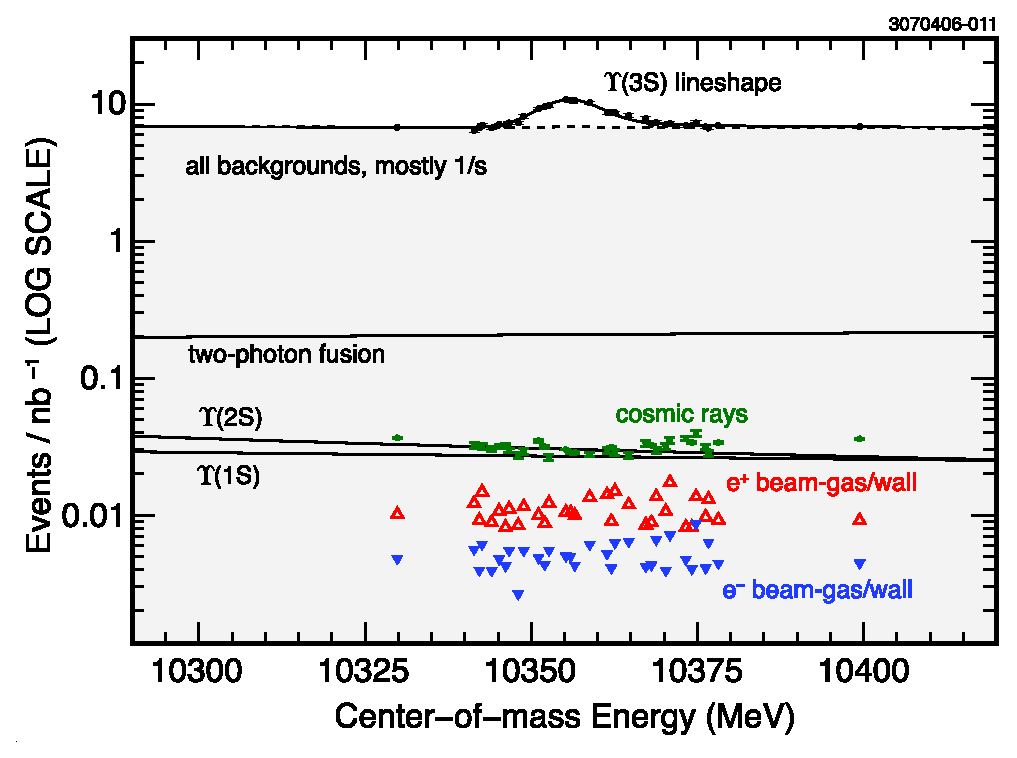
\includegraphics[width=0.8\linewidth]{backgrounds}
\end{center}
\end{slidemap}

%%%%%%%%%%%%%%%%%%%%%%%%%%%%%%%%%%%%%%%%%%%%%%%%%%%%%%%%%%%%%%%%%%%%%%%%%%%%%%

\begin{slidemap}[technique & efficiency & backgrounds & \textcolor{blue}{luminosity} & energy & fits & results & theory]

\vfill
Integrated luminosity = observed Bhabhas / efficiency-weighted Bhabha cross-section

\vfill
\begin{center}
Points are data, solid histograms are scaled Monte Carlo (Babayaga)

\begin{tabular}{p{0.45\linewidth} p{0.45\linewidth}}
\begin{minipage}{\linewidth}
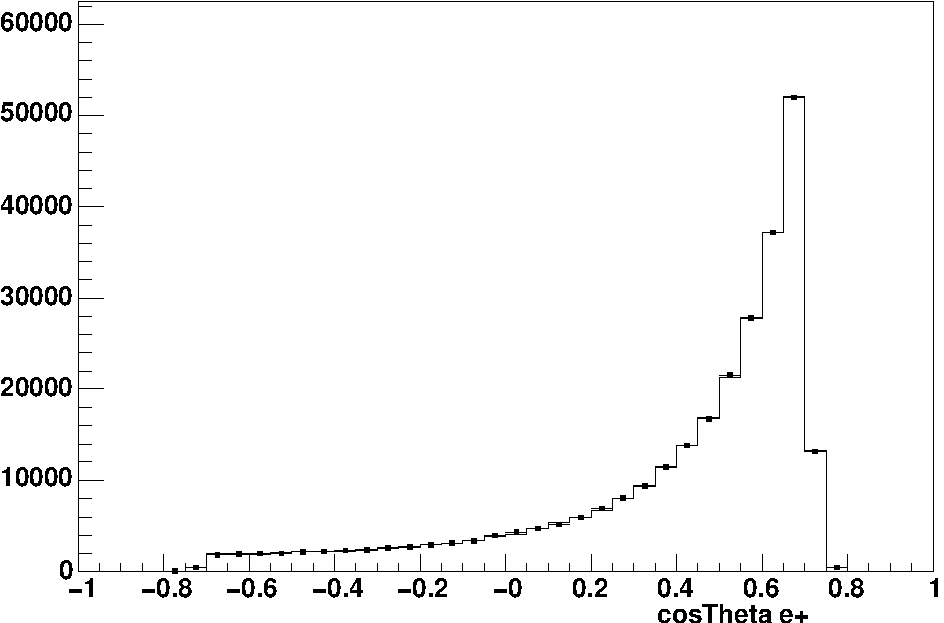
\includegraphics[width=\linewidth]{luminosity_costheta}
\end{minipage} &
\begin{minipage}{\linewidth}
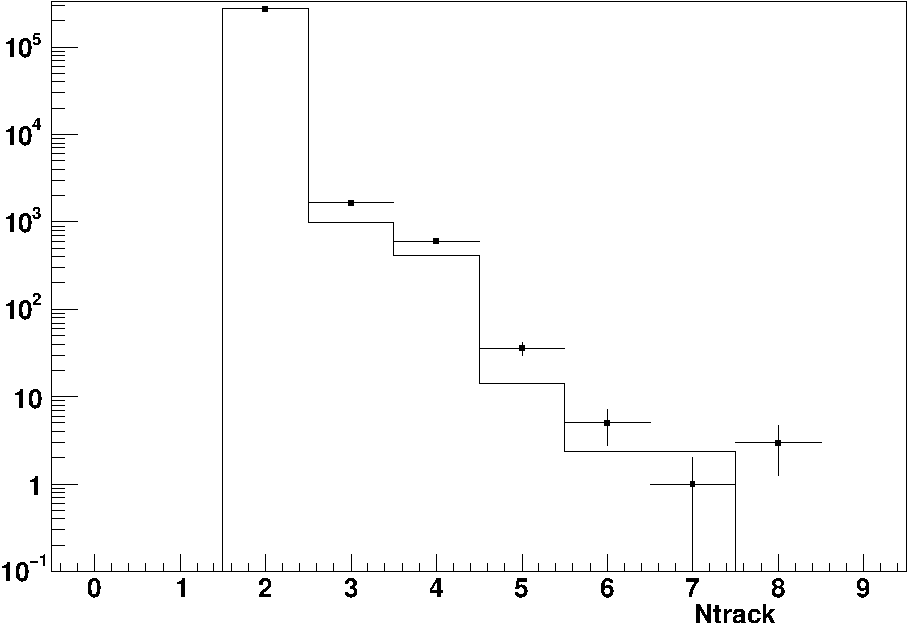
\includegraphics[width=\linewidth]{luminosity_tracks}
\end{minipage} \\
\begin{minipage}{\linewidth}
\begin{center}
\Huge cos$\theta$ of the $e^+$
\end{center}
\end{minipage} &
\begin{minipage}{\linewidth}
\begin{center}
\Huge Number of Observed Tracks
\end{center}
\end{minipage}
\end{tabular}
\end{center}

\vfill
\end{slidemap}

%%%%%%%%%%%%%%%%%%%%%%%%%%%%%%%%%%%%%%%%%%%%%%%%%%%%%%%%%%%%%%%%%%%%%%%%%%%%%%

\begin{slidemap}[technique & efficiency & backgrounds & \textcolor{blue}{luminosity} & energy & fits & results & theory]
Overall scale of $e^+e^-$ calculation is checked by $\mu^+\mu^-$ and $\gamma\gamma$

\vfill
\begin{center}
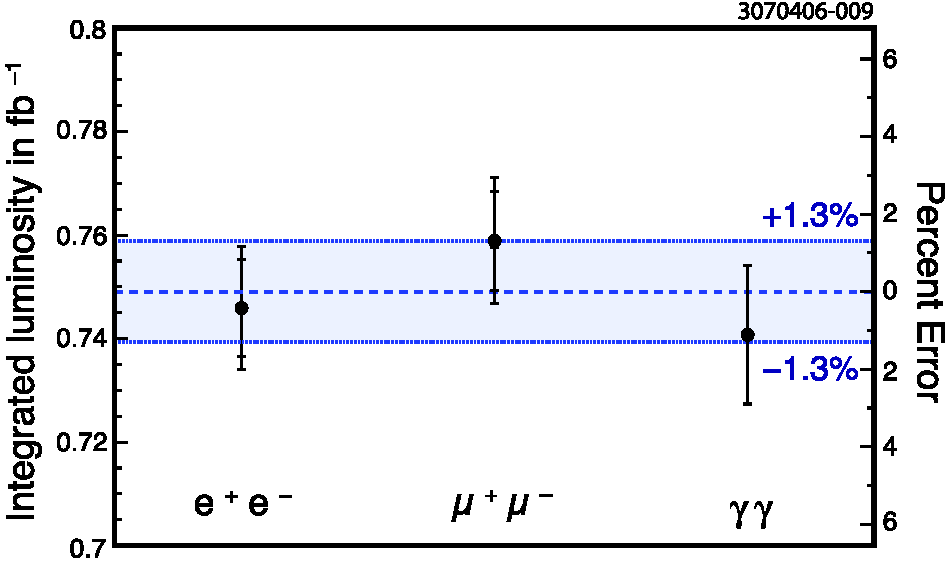
\includegraphics[width=0.9\linewidth]{luminosity}
\end{center}
\vfill
\end{slidemap}

%%%%%%%%%%%%%%%%%%%%%%%%%%%%%%%%%%%%%%%%%%%%%%%%%%%%%%%%%%%%%%%%%%%%%%%%%%%%%%

\begin{slidemap}[technique & efficiency & backgrounds & luminosity & \textcolor{blue}{energy} & fits & results & theory]
\begin{tabular}{p{0.6\linewidth} p{0.37\linewidth}}
  \begin{minipage}{\linewidth}
    \begin{minipage}{0.9\linewidth}
      \begin{itemize}\setlength{\itemsep}{0.75 cm}

	\item Beam energy determined by dipole magnet measurement

	\item Calibration drifts with time (0.5~MeV/month)

	\item Each resonance completely scanned in 48 hours (repeated
	scans for statistical precision)

        \item Measurements alternated above and below resonance peak

        \item Repeated point of high slope ({\color{red} 1 \& 5}):
        convert cross-section reproducibility into beam energy reproducibility

	\item $\Rightarrow$ 0.07~MeV uncertainty in center-of-mass differences, 0.2\% in $\Gamma_{ee}$

	\end{itemize}
    \end{minipage}

  \end{minipage} &
  \begin{minipage}{\linewidth}
    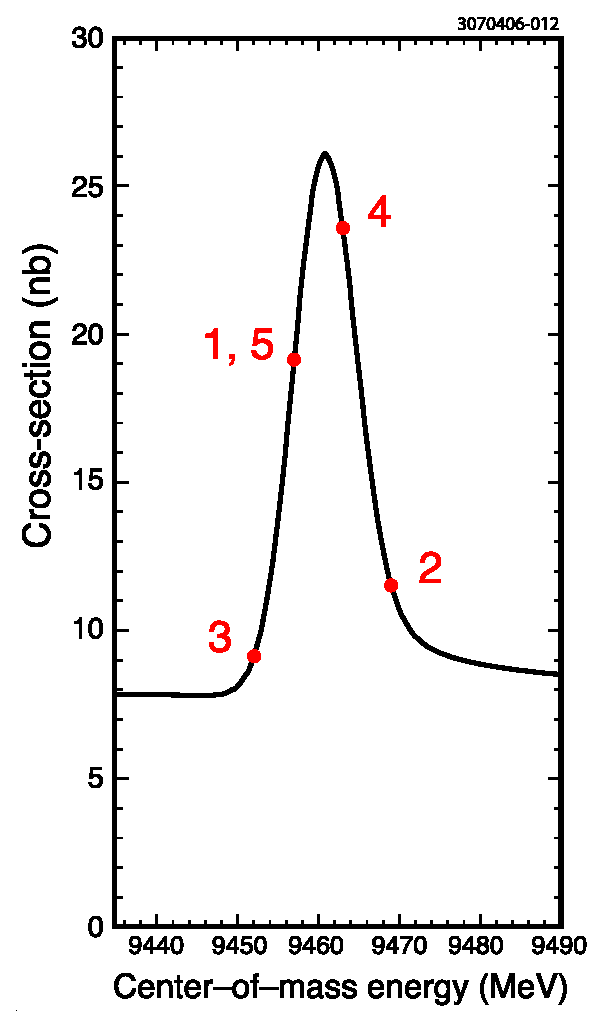
\includegraphics[width=\linewidth]{scanorder}
  \end{minipage}
\end{tabular}

\vfill
\end{slidemap}

%%%%%%%%%%%%%%%%%%%%%%%%%%%%%%%%%%%%%%%%%%%%%%%%%%%%%%%%%%%%%%%%%%%%%%%%%%%%%%

\begin{slidemap}[technique & efficiency & backgrounds & luminosity & energy & \textcolor{blue}{fits} & results & theory]
\vfill
\begin{center}
{\boldmath
\hspace{0.5 cm} \begin{tabular}{c c c}
  $\chi^2/N_{\mbox{\Large dof}} = 1.3$ \mbox{\hspace{2.7 cm}} & $\chi^2/N_{\mbox{\Large dof}} = 1.6$ & \mbox{\hspace{2.9 cm}} $\chi^2/N_{\mbox{\Large dof}} = 1.0$
\end{tabular}}
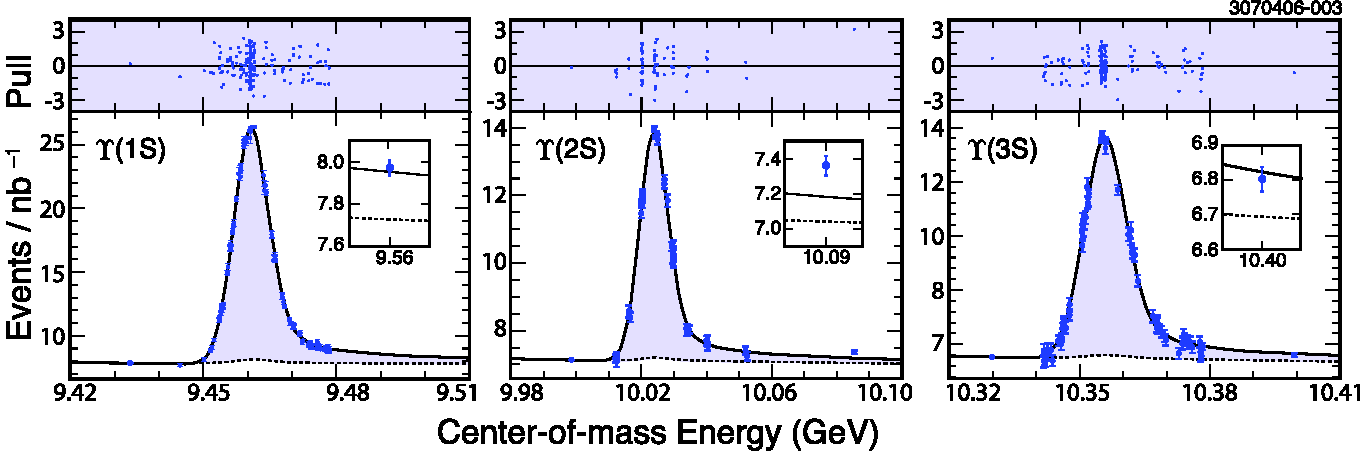
\includegraphics[width=\linewidth, height=14 cm]{fits}
\end{center}
\vfill
\end{slidemap}

%%%%%%%%%%%%%%%%%%%%%%%%%%%%%%%%%%%%%%%%%%%%%%%%%%%%%%%%%%%%%%%%%%%%%%%%%%%%%%

\begin{slidemap}[technique & efficiency & backgrounds & luminosity & energy & \textcolor{blue}{fits} & results & theory]
{\Huge \bf Lineshape Distortions}

\begin{itemize}

  \item Non-Gaussian beam energy spread?  {\bf No,} not observed with 0.3\% statistical precision

  \item Variable beam energy spread?  {\bf Yes,} we observed 1\% variation in a month

  \item Interference between $e^+e^- \to \Upsilon \to$ hadrons and $e^+e^- \to$ hadrons?  {\bf Yes!}

\end{itemize}

\vfill
\begin{center}
\begin{tabular}{p{0.35\linewidth} c p{0.4\linewidth}}
\begin{minipage}{\linewidth}
\begin{center}
Exaggerated Interference

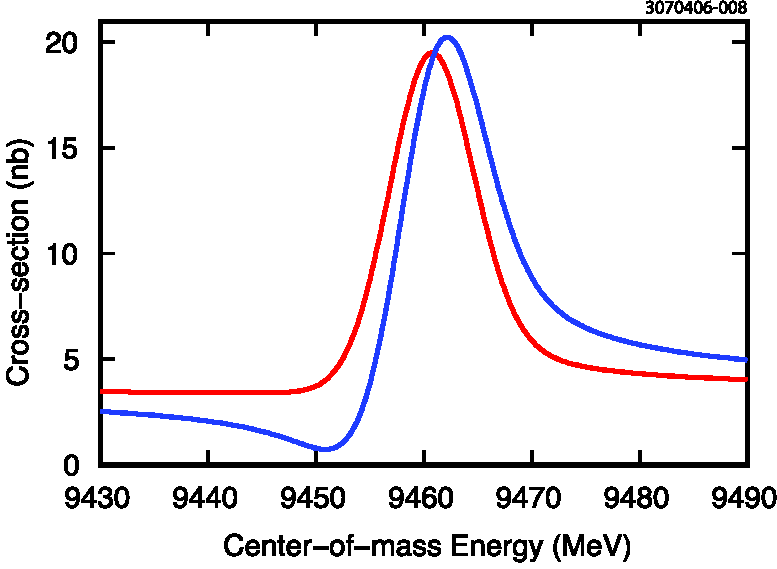
\includegraphics[width=\linewidth]{interference_cartoon}
\end{center}
\end{minipage} & \hspace{1 cm} &
\begin{minipage}{\linewidth}
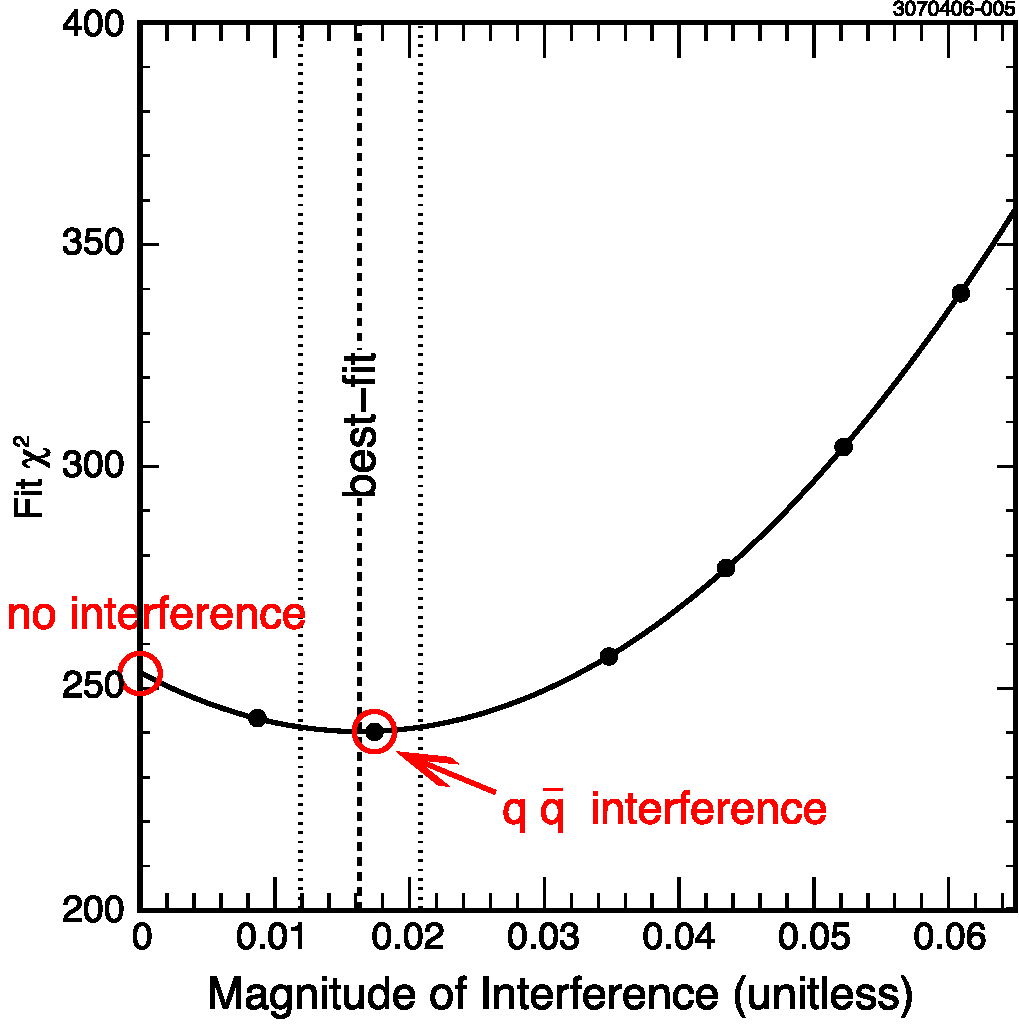
\includegraphics[width=\linewidth]{interference_fit_fixedphase}
\end{minipage}
\end{tabular}
\end{center}

\vfill
\end{slidemap}

%%%%%%%%%%%%%%%%%%%%%%%%%%%%%%%%%%%%%%%%%%%%%%%%%%%%%%%%%%%%%%%%%%%%%%%%%%%%%%

\begin{slidemap}[technique & efficiency & backgrounds & luminosity & energy & fits & \textcolor{blue}{results} & theory]
\mbox{ } \hfill {\color{blue} $^*$Common to all resonances}

\vfill
\begin{center}
  \renewcommand{\arraystretch}{1.3}
  \begin{tabular}{l c c c}
    \hline\hline Contribution to $\Gamma_{ee}$ & \hspace{0.5 cm}$\Upsilon(1S)$\hspace{0.5 cm} & \hspace{0.5 cm}$\Upsilon(2S)$\hspace{0.5 cm} & \hspace{0.5 cm}$\Upsilon(3S)$\hspace{0.5 cm} \\\hline
    Correction for leptonic modes        	   & 0.2\%  & 0.2\%  & 0.3\%  \\
    {\color{blue} Hadronic efficiency$^*$} & {\color{blue} 0.5\%}  & {\color{blue} 0.5\%}  & {\color{blue} 0.5\%}  \\
    $Xe^+e^-$, $X\mu^+\mu^-$ correction  	   & 0      & 0.15\% & 0.13\% \\
    {\color{blue} Overall luminosity scale$^*$} & {\color{blue} 1.3\%}  & {\color{blue} 1.3\%}  & {\color{blue} 1.3\%}  \\
    Bhabha/$\gamma\gamma$ inconsistency  	   & 0.4\%  & 0.4\%  & 0.4\%  \\
    Beam energy measurement drift \hspace{0.5 cm}  & 0.2\%  & 0.2\%  & 0.2\%  \\
    Fit function shape                   	   & 0.1\%  & 0.1\%  & 0.1\%  \\
    $\chi^2$ inconsistency               	   & 0.2\%  & 0.6\%  & 0      \\\hline
    Total systematic uncertainty         	   & {\color{red} 1.5\%}  & {\color{red} 1.6\%}  & {\color{red} 1.5\%}  \\
    Statistical uncertainty              	   & 0.3\%  & 0.7\%  & 1.0\%  \\\hline
    Total                                	   & {\color{red} 1.5\%}  & {\color{red} 1.8\%}  & {\color{red} 1.8\%}  \\\hline\hline
  \end{tabular}
\end{center}

\vfill
\end{slidemap}

%%%%%%%%%%%%%%%%%%%%%%%%%%%%%%%%%%%%%%%%%%%%%%%%%%%%%%%%%%%%%%%%%%%%%%%%%%%%%%

\begin{slidemap}[technique & efficiency & backgrounds & luminosity & energy & fits & \textcolor{blue}{results} & theory]
\begin{center}
\renewcommand{\arraystretch}{1.6}
\begin{tabular}{c c c c}
%%   \boldmath $\Gamma_{ee}\Gamma_\subs{had}/\Gamma_\subs{tot}(1S)$ & \mbox{\hspace{0.25 cm}} = \mbox{\hspace{0.25 cm}} & 1.252 $\pm$ 0.004 $\pm$ 0.019 keV & \mbox{\hspace{0.5 cm}} 1.6\% \mbox{\hspace{0.5 cm}}  \\
%%   \boldmath $\Gamma_{ee}\Gamma_\subs{had}/\Gamma_\subs{tot}(2S)$ & = & 0.581 $\pm$ 0.004 $\pm$ 0.009 keV & 1.7\% \\
%%   \boldmath $\Gamma_{ee}\Gamma_\subs{had}/\Gamma_\subs{tot}(3S)$ & = & 0.413 $\pm$ 0.004 $\pm$ 0.006 keV & 1.7\% \\\hline

  \boldmath $\Gamma_{ee}(1S)$ & \mbox{\hspace{0.25 cm}} = \mbox{\hspace{0.25 cm}} & 1.354 $\pm$ 0.004 $\pm$ 0.020 keV & \mbox{\hspace{0.5 cm}} 1.5\% \mbox{\hspace{0.5 cm}} \\
  \boldmath $\Gamma_{ee}(2S)$ & = & 0.619 $\pm$ 0.004 $\pm$ 0.010 keV & 1.8\% \\
  \boldmath $\Gamma_{ee}(3S)$ & = & 0.446 $\pm$ 0.004 $\pm$ 0.007 keV & 1.8\% \\\hline

  \boldmath $\Gamma_{ee}(2S)/\Gamma_{ee}(1S)$ & = & 0.457 $\pm$ 0.004 $\pm$ 0.004 keV & 1.2\% \\
  \boldmath $\Gamma_{ee}(3S)/\Gamma_{ee}(1S)$ & = & 0.329 $\pm$ 0.003 $\pm$ 0.003 keV & 1.3\% \\
  \boldmath $\Gamma_{ee}(3S)/\Gamma_{ee}(2S)$ & = & 0.720 $\pm$ 0.009 $\pm$ 0.007 keV & 1.6\% \\\hline

  \boldmath $\Gamma(1S)$ & = & 54.4 $\pm$ 0.2 $\pm$ 0.8 $\pm$ 1.6 keV & 3.3\% \\
  \boldmath $\Gamma(2S)$ & = & 30.5 $\pm$ 0.2 $\pm$ 0.5 $\pm$ 1.3 keV & 4.6\% \\
  \boldmath $\Gamma(3S)$ & = & 18.6 $\pm$ 0.2 $\pm$ 0.3 $\pm$ $\underbrace{\mbox{0.9}}_{{\mathcal B}_{\mu\mu}}$ keV & 5.2\% \\

\end{tabular}
\end{center}

\vfill
{\Large $\Gamma_{ee}$: J.L.~Rosner {\it et al.} (CLEO Collaboration) Phys.\ Rev.\ Lett.\ {\bf 96}, 092003 (2006) \\
${\mathcal B}_{\mu\mu}$: G.S.~Adams {\it et al.} (CLEO Collaboration), Phys.\ Rev.\ Lett.\ {\bf 94}, 012001 (2005)}
\end{slidemap}

%%%%%%%%%%%%%%%%%%%%%%%%%%%%%%%%%%%%%%%%%%%%%%%%%%%%%%%%%%%%%%%%%%%%%%%%%%%%%%

\begin{slidemap}[technique & efficiency & backgrounds & luminosity & energy & fits & \textcolor{blue}{results} & theory]
\begin{center}
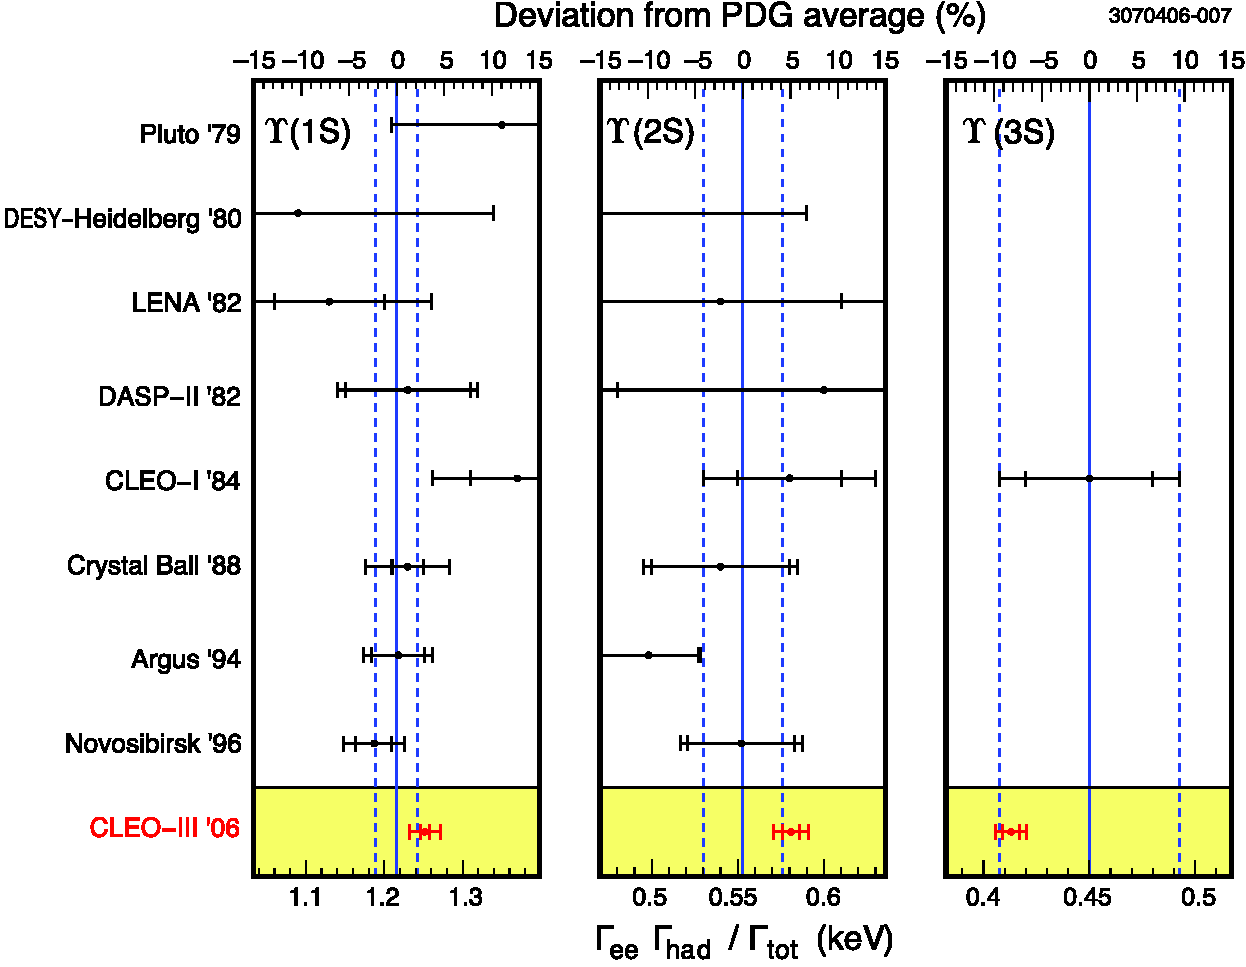
\includegraphics[width=0.77\linewidth]{history}
\end{center}
\vfill
\end{slidemap}

%%%%%%%%%%%%%%%%%%%%%%%%%%%%%%%%%%%%%%%%%%%%%%%%%%%%%%%%%%%%%%%%%%%%%%%%%%%%%%

\begin{slidemap}[technique & efficiency & backgrounds & luminosity & energy & fits & results & \textcolor{blue}{theory}]
{\Huge \bf \boldmath Lattice QCD Calculations of $\Gamma_{ee}$}

\begin{center}

\begin{tabular}{r l}
\textcolor{black}{Summer 2005:} & \textcolor{black}{10\%-level prediction of $\Gamma_{ee}(2S)/\Gamma_{ee}(1S)$ ratio} \hspace{3 cm} \\
Later this summer: & few-percent ratios, 10\% absolute $\Gamma_{ee}$
\end{tabular}

\vfill
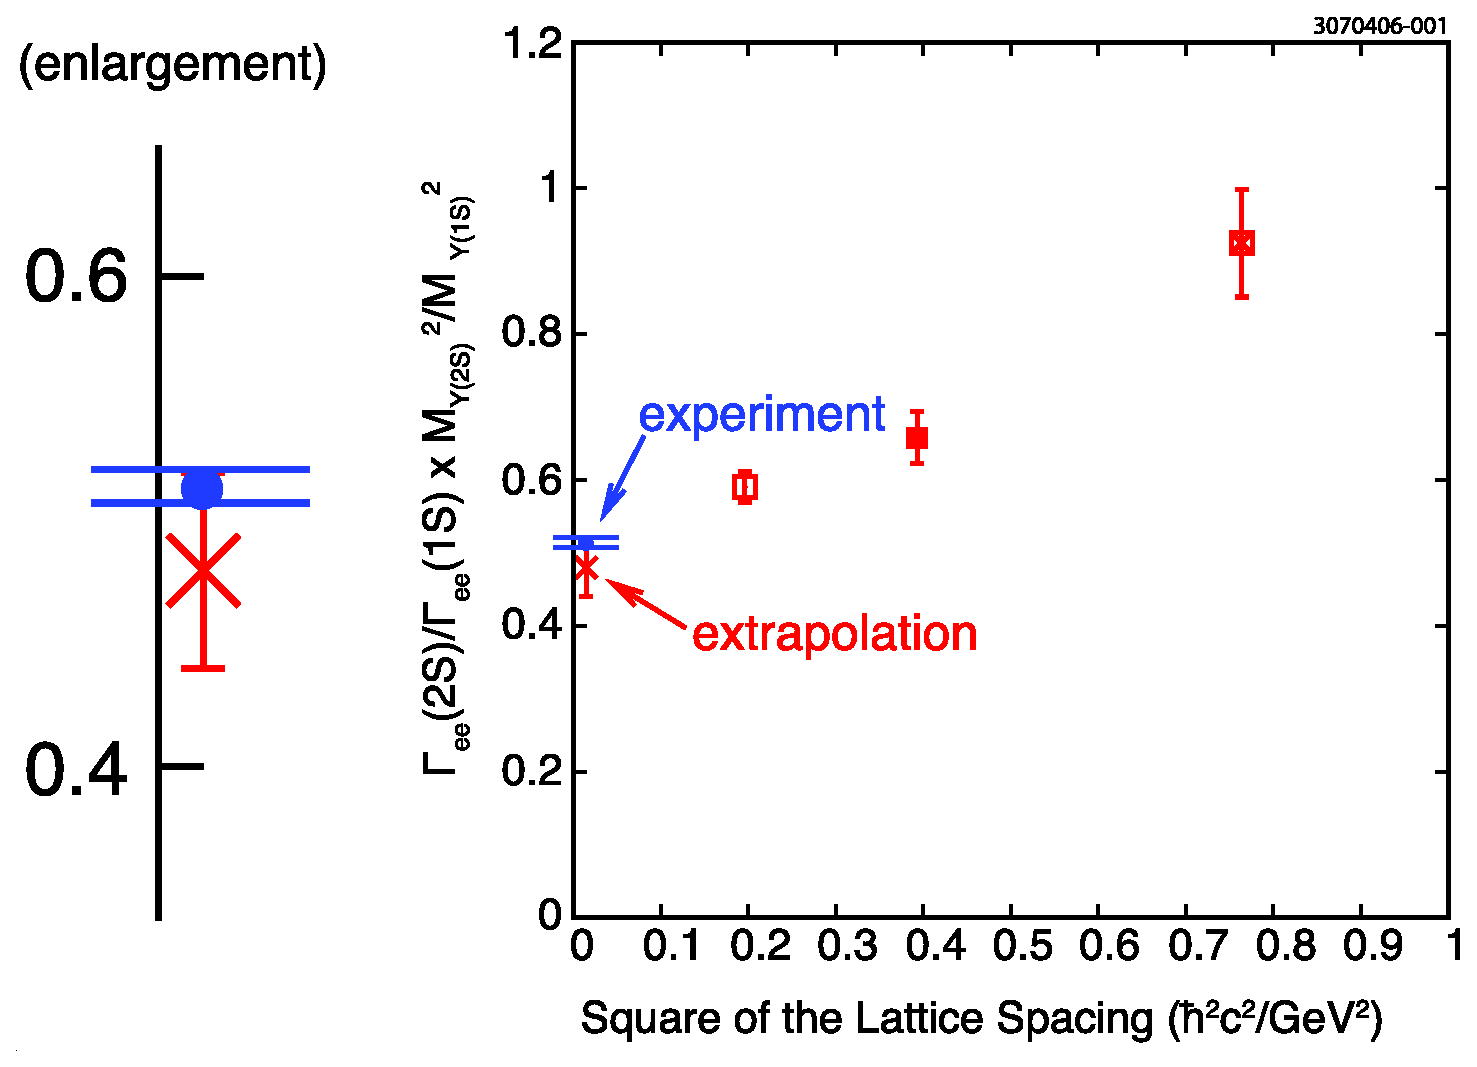
\includegraphics[width=0.65\linewidth]{comparison_lattice}

\end{center}

{\Large A.~Gray {\it et al.} (HPQCD Collaboration), Phys.\ Rev.\ D {\bf 72}, 094507 (2005)}
\end{slidemap}

%%%%%%%%%%%%%%%%%%%%%%%%%%%%%%%%%%%%%%%%%%%%%%%%%%%%%%%%%%%%%%%%%%%%%%%%%%%%%%

\begin{slidemap}[technique & efficiency & backgrounds & luminosity & energy & fits & results & \textcolor{blue}{theory}]
{\Huge \bf Why the Steep Dependence on Lattice Spacing?}

\vfill
Decay constants sample wavefunction at the origin, which is discretized

\begin{center}
\begin{tabular}{p{0.3\linewidth} p{0.1\linewidth} p{0.3\linewidth}}
\begin{minipage}{\linewidth}

\includegraphics[width=\linewidth, trim=0 60 0 60, clip=true]{fuzzyloose}
\end{minipage} &
\begin{minipage}{\linewidth}
\boldmath $\longrightarrow$
\end{minipage} &
\begin{minipage}{\linewidth}
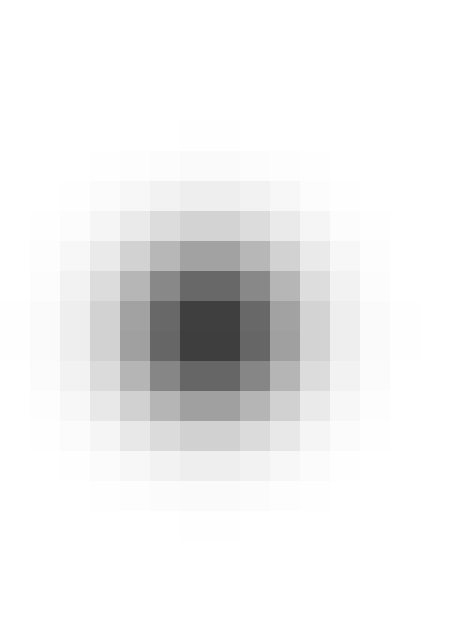
\includegraphics[width=\linewidth, trim=0 60 0 60, clip=true]{fuzzyloose-digital}
\end{minipage}
\end{tabular}
\end{center}

\vfill
$\Upsilon$ is a small meson, making discretization more severe

\vfill
\end{slidemap}

%%%%%%%%%%%%%%%%%%%%%%%%%%%%%%%%%%%%%%%%%%%%%%%%%%%%%%%%%%%%%%%%%%%%%%%%%%%%%%

\begin{slidemap}[technique & efficiency & backgrounds & luminosity & energy & fits & results & \textcolor{blue}{theory}]
{\Huge \bf \boldmath How Relevant is this Test to $f_B$?}

\vfill
\begin{center}
\begin{tabular}{p{10 cm} p{1.8 cm} p{10 cm}}
\begin{minipage}{\linewidth}
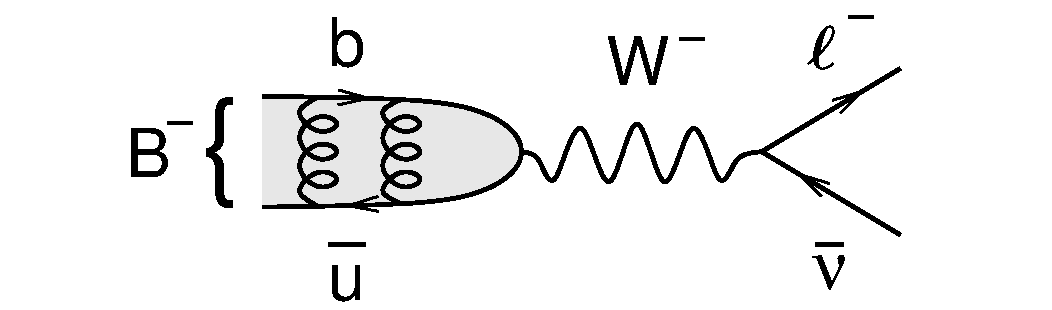
\includegraphics[width=\linewidth]{diagram_Btolnu}
\end{minipage} &
\begin{minipage}{\linewidth}
vs.
\end{minipage} &
\begin{minipage}{\linewidth}
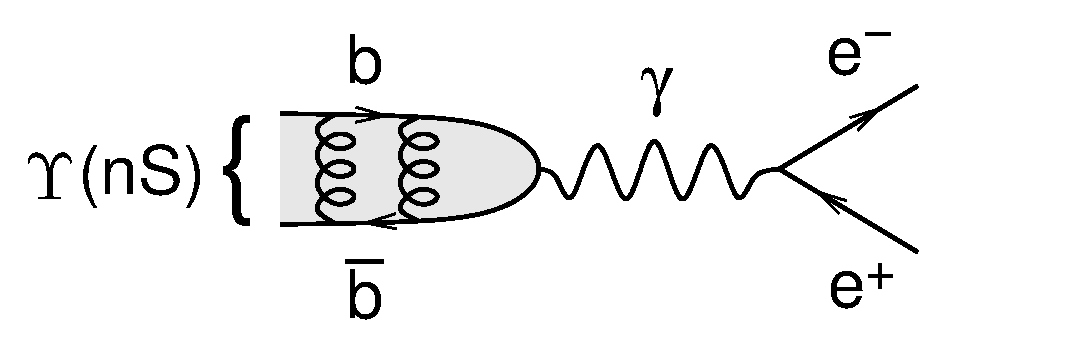
\includegraphics[width=\linewidth]{diagram_GeeU}
\end{minipage}
\end{tabular}
\end{center}

\vfill
\begin{itemize}\setlength{\itemsep}{0.5 cm}

  \item $\Gamma_{ee}$ and $f_B$ calculations share the same NRQCD action and staggered-quark formalism

  \item Discretization errors in $f_B$ are smaller than discretization errors in $\Gamma_{ee}$

  \item Though $\Upsilon$ couples to vector current, the factor this introduces cancels in ratios of $\Gamma_{ee}$

\end{itemize}

\vfill
Compliments $f_D$ and $\Gamma(\psi \to e^+e^-)$ tests

\vfill
\end{slidemap}

%%%%%%%%%%%%%%%%%%%%%%%%%%%%%%%%%%%%%%%%%%%%%%%%%%%%%%%%%%%%%%%%%%%%%%%%%%%%%%

\begin{slide}
{\Huge \bf \boldmath CLEO has also measured $\Gamma_{ee}$ for $J/\psi$ and $\psi(2S)$}

\vspace{0.75 cm}
Measured with initial-state radiation, rather than scans

\vfill
\begin{center}
\begin{tabular}{p{0.45\linewidth} p{0.45\linewidth}}
\begin{minipage}{\linewidth} \begin{center} \bf Scan Method \end{center} \end{minipage} &
\begin{minipage}{\linewidth} \begin{center} \bf ISR Method \end{center} \end{minipage} \\
\begin{minipage}{\linewidth} \begin{center} 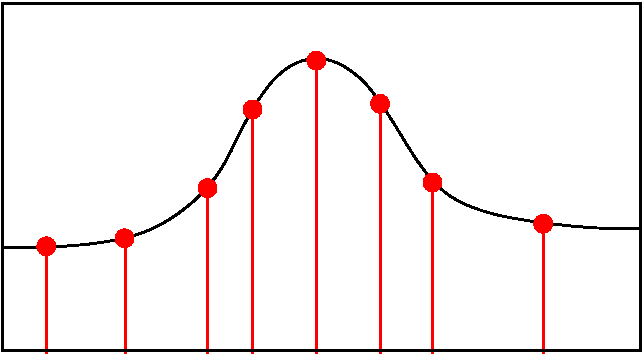
\includegraphics[width=0.8\linewidth]{signify_scan} \end{center} \end{minipage} &
\begin{minipage}{\linewidth} \begin{center} 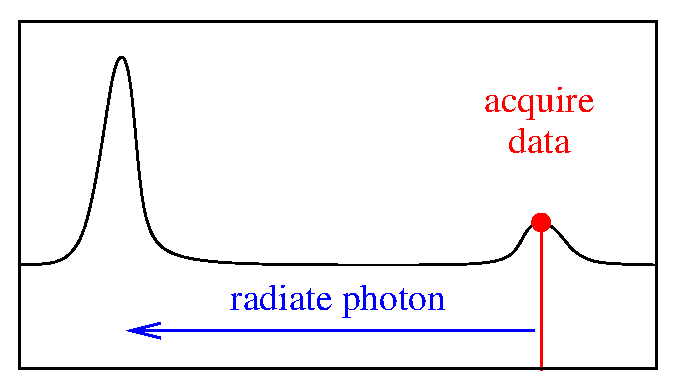
\includegraphics[width=0.8\linewidth]{signify_isr} \end{center} \end{minipage} \\
\begin{minipage}{\linewidth}

\vspace{0.5 cm}
\begin{itemize}

  \item Requires dedicated scans

  \item Measure inclusive cross-section

  \item Requires detailed understanding of the lineshape

\end{itemize}
\end{minipage} &
\begin{minipage}{\linewidth}

\vspace{0.5 cm}
\begin{itemize}

  \item Select events from a large dataset

  \item Distinctive final states ($\pi^+\pi^- J/\psi$)

  \item Requires precise knowledge of ${\mathcal B}(\pi^+\pi^- J/\psi)$

\end{itemize}
\end{minipage}

\end{tabular}
\end{center}

\vfill
\end{slide}

%%%%%%%%%%%%%%%%%%%%%%%%%%%%%%%%%%%%%%%%%%%%%%%%%%%%%%%%%%%%%%%%%%%%%%%%%%%%%%

\begin{slide}
{\Huge \bf \boldmath $\Gamma_{ee}$ for $J/\psi$ and $\psi(2S)$}

\begin{center}
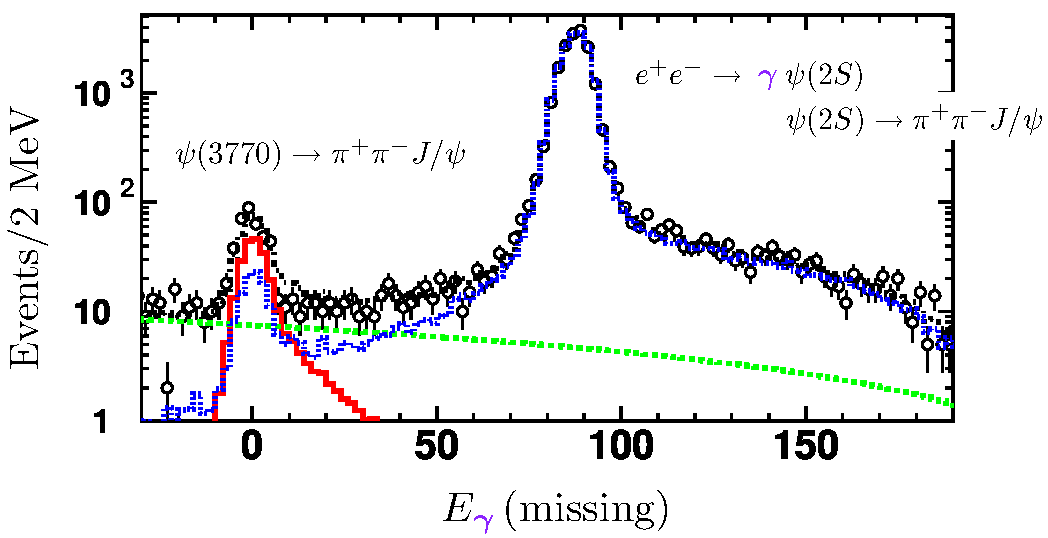
\includegraphics[width=0.8\linewidth]{psi_gamee2}

\vfill
\renewcommand{\arraystretch}{1.4}
\begin{tabular}{c c c c}
  \boldmath $\Gamma_{ee}(J/\psi)$ & \mbox{\hspace{0.25 cm}} = \mbox{\hspace{0.25 cm}} & 5.68 $\pm$ 0.11 $\pm$ 0.13 keV & \mbox{\hspace{0.5 cm}} 3.0\% \mbox{\hspace{0.5 cm}} \\
  \boldmath $\Gamma_{ee}(\psi(2S))$ & = & 2.54 $\pm$ 0.03 $\pm$ 0.11 keV & 4.5\% \\

  \boldmath $\Gamma_{ee}(\psi(2S))/\Gamma_{ee}(J/\psi)$ & = & 0.45 $\pm$ 0.01 $\pm$ 0.02 keV & 5.0\% \\
\end{tabular}
\end{center}

\vfill
{\Large
N.E.~Adam (CLEO Collaboration) Phys.\ Rev.\ Lett.\ {\bf 96} 082004
(2006) and \\ G.S.~Adams (CLEO Collaboration) Phys.\ Rev.\ {\bf D73}
051103 (2006)}
\end{slide}

%%%%%%%%%%%%%%%%%%%%%%%%%%%%%%%%%%%%%%%%%%%%%%%%%%%%%%%%%%%%%%%%%%%%%%%%%%%%%%

\begin{slide}
{\Huge \bf Summary}

\vspace{0.75 cm}
CLEO provides key tests of Lattice QCD relevant for $f_B$

\vfill
\begin{center}
  \renewcommand{\arraystretch}{1.5}
  \begin{tabular}{| c | c c c |}
    \hline & heavy-heavy & \mbox{\hspace{1 cm}} & heavy-light \\\hline
    \mbox{\hspace{0.5 cm}} bottom \mbox{\hspace{0.5 cm}} & $\Gamma_{ee}$ for $\Upsilon$ & & $f_B$ \\
    & & & \\
    \mbox{\hspace{0.5 cm}} charm \mbox{\hspace{0.5 cm}} & $\Gamma_{ee}$ for $\psi$ & & $f_D$ \\\hline
  \end{tabular}
\end{center}

\vfill
$\Gamma_{ee}$ for $\Upsilon(1S)$, $\Upsilon(2S)$, $\Upsilon(3S)$, and ratios have better than 2\% precision

\vfill
Few-percent calculations of $\Gamma_{ee}$ from Lattice QCD are expected this summer

\vfill
If they compare favorably, we can have greater confidence in $V_{td}$ determinations \\
and our understanding of QCD in general

\vfill
\end{slide}

%%%%%%%%%%%%%%%%%%%%%%%%%%%%%%%%%%%%%%%%%%%%%%%%%%%%%%%%%%%%%%%%%%%%%%%%%%%%%%

%% \begin{slide}
%% {\Huge \bf Title}

%% \vspace{0.75 cm}
%% Stuff

%% \end{slide}

%%%%%%%%%%%%%%%%%%%%%%%%%%%%%%%%%%%%%%%%%%%%%%%%%%%%%%%%%%%%%%%%%%%%%%%%%%%%%%

%% \begin{slide}
%% {\Huge \bf Title}

%% \vspace{0.75 cm}
%% Stuff

%% \end{slide}

%%%%%%%%%%%%%%%%%%%%%%%%%%%%%%%%%%%%%%%%%%%%%%%%%%%%%%%%%%%%%%%%%%%%%%%%%%%%%%

%% \begin{slide}
%% {\Huge \bf Title}

%% \vspace{0.75 cm}
%% Stuff

%% \end{slide}

%%%%%%%%%%%%%%%%%%%%%%%%%%%%%%%%%%%%%%%%%%%%%%%%%%%%%%%%%%%%%%%%%%%%%%%%%%%%%%

%% \begin{slide}
%% {\Huge \bf Title}

%% \vspace{0.75 cm}
%% Stuff

%% \end{slide}

%%%%%%%%%%%%%%%%%%%%%%%%%%%%%%%%%%%%%%%%%%%%%%%%%%%%%%%%%%%%%%%%%%%%%%%%%%%%%%

%% \begin{slide}
%% {\Huge \bf Title}

%% \vspace{0.75 cm}
%% Stuff

%% \end{slide}

%%%%%%%%%%%%%%%%%%%%%%%%%%%%%%%%%%%%%%%%%%%%%%%%%%%%%%%%%%%%%%%%%%%%%%%%%%%%%%

%% \begin{slide}
%% {\Huge \bf Title}

%% \vspace{0.75 cm}
%% Stuff

%% \end{slide}

%%%%%%%%%%%%%%%%%%%%%%%%%%%%%%%%%%%%%%%%%%%%%%%%%%%%%%%%%%%%%%%%%%%%%%%%%%%%%%

%% \begin{slide}
%% {\Huge \bf Title}

%% \vspace{0.75 cm}
%% Stuff

%% \end{slide}

%%%%%%%%%%%%%%%%%%%%%%%%%%%%%%%%%%%%%%%%%%%%%%%%%%%%%%%%%%%%%%%%%%%%%%%%%%%%%%

%% \begin{slide}
%% {\Huge \bf Title}

%% \vspace{0.75 cm}
%% Stuff

%% \end{slide}

%%%%%%%%%%%%%%%%%%%%%%%%%%%%%%%%%%%%%%%%%%%%%%%%%%%%%%%%%%%%%%%%%%%%%%%%%%%%%%

%% \begin{slide}
%% {\Huge \bf Title}

%% \vspace{0.75 cm}
%% Stuff

%% \end{slide}

%%%%%%%%%%%%%%%%%%%%%%%%%%%%%%%%%%%%%%%%%%%%%%%%%%%%%%%%%%%%%%%%%%%%%%%%%%%%%%

%% \begin{slide}
%% {\Huge \bf Title}

%% \vspace{0.75 cm}
%% Stuff

%% \end{slide}

%%%%%%%%%%%%%%%%%%%%%%%%%%%%%%%%%%%%%%%%%%%%%%%%%%%%%%%%%%%%%%%%%%%%%%%%%%%%%%

%% \begin{slide}
%% {\Huge \bf Title}

%% \vspace{0.75 cm}
%% Stuff

%% \end{slide}

%%%%%%%%%%%%%%%%%%%%%%%%%%%%%%%%%%%%%%%%%%%%%%%%%%%%%%%%%%%%%%%%%%%%%%%%%%%%%%

%% \begin{slide}
%% {\Huge \bf Title}

%% \vspace{0.75 cm}
%% Stuff

%% \end{slide}

%%%%%%%%%%%%%%%%%%%%%%%%%%%%%%%%%%%%%%%%%%%%%%%%%%%%%%%%%%%%%%%%%%%%%%%%%%%%%%

%% \begin{slide}
%% {\Huge \bf Title}

%% \vspace{0.75 cm}
%% Stuff

%% \end{slide}

%%%%%%%%%%%%%%%%%%%%%%%%%%%%%%%%%%%%%%%%%%%%%%%%%%%%%%%%%%%%%%%%%%%%%%%%%%%%%%

%% \begin{slide}
%% {\Huge \bf Title}

%% \vspace{0.75 cm}
%% Stuff

%% \end{slide}

%%%%%%%%%%%%%%%%%%%%%%%%%%%%%%%%%%%%%%%%%%%%%%%%%%%%%%%%%%%%%%%%%%%%%%%%%%%%%%

%% \begin{slide}
%% {\Huge \bf Title}

%% \vspace{0.75 cm}
%% Stuff

%% \end{slide}

%%%%%%%%%%%%%%%%%%%%%%%%%%%%%%%%%%%%%%%%%%%%%%%%%%%%%%%%%%%%%%%%%%%%%%%%%%%%%%

%% \begin{slide}
%% {\Huge \bf Title}

%% \vspace{0.75 cm}
%% Stuff

%% \end{slide}

%%%%%%%%%%%%%%%%%%%%%%%%%%%%%%%%%%%%%%%%%%%%%%%%%%%%%%%%%%%%%%%%%%%%%%%%%%%%%%

%% \begin{slide}
%% {\Huge \bf Title}

%% \vspace{0.75 cm}
%% Stuff

%% \end{slide}

%%%%%%%%%%%%%%%%%%%%%%%%%%%%%%%%%%%%%%%%%%%%%%%%%%%%%%%%%%%%%%%%%%%%%%%%%%%%%%

%% \begin{slide}
%% {\Huge \bf Title}

%% \vspace{0.75 cm}
%% Stuff

%% \end{slide}

%%%%%%%%%%%%%%%%%%%%%%%%%%%%%%%%%%%%%%%%%%%%%%%%%%%%%%%%%%%%%%%%%%%%%%%%%%%%%%

%% \begin{slide}
%% {\Huge \bf Title}

%% \vspace{0.75 cm}
%% Stuff

%% \end{slide}

%%%%%%%%%%%%%%%%%%%%%%%%%%%%%%%%%%%%%%%%%%%%%%%%%%%%%%%%%%%%%%%%%%%%%%%%%%%%%%

%% \begin{slide}
%% {\Huge \bf Title}

%% \vspace{0.75 cm}
%% Stuff

%% \end{slide}

%%%%%%%%%%%%%%%%%%%%%%%%%%%%%%%%%%%%%%%%%%%%%%%%%%%%%%%%%%%%%%%%%%%%%%%%%%%%%%

%% \begin{slide}
%% {\Huge \bf Title}

%% \vspace{0.75 cm}
%% Stuff

%% \end{slide}

%%%%%%%%%%%%%%%%%%%%%%%%%%%%%%%%%%%%%%%%%%%%%%%%%%%%%%%%%%%%%%%%%%%%%%%%%%%%%%

%% \begin{slide}
%% {\Huge \bf Title}

%% \vspace{0.75 cm}
%% Stuff

%% \end{slide}

%%%%%%%%%%%%%%%%%%%%%%%%%%%%%%%%%%%%%%%%%%%%%%%%%%%%%%%%%%%%%%%%%%%%%%%%%%%%%%

%% \begin{slide}
%% {\Huge \bf Title}

%% \vspace{0.75 cm}
%% Stuff

%% \end{slide}

%%%%%%%%%%%%%%%%%%%%%%%%%%%%%%%%%%%%%%%%%%%%%%%%%%%%%%%%%%%%%%%%%%%%%%%%%%%%%%

%% \begin{slide}
%% {\Huge \bf Title}

%% \vspace{0.75 cm}
%% Stuff

%% \end{slide}

%%%%%%%%%%%%%%%%%%%%%%%%%%%%%%%%%%%%%%%%%%%%%%%%%%%%%%%%%%%%%%%%%%%%%%%%%%%%%%

%% \begin{slide}
%% {\Huge \bf Title}

%% \vspace{0.75 cm}
%% Stuff

%% \end{slide}

%%%%%%%%%%%%%%%%%%%%%%%%%%%%%%%%%%%%%%%%%%%%%%%%%%%%%%%%%%%%%%%%%%%%%%%%%%%%%%

%% \begin{slide}
%% {\Huge \bf Title}

%% \vspace{0.75 cm}
%% Stuff

%% \end{slide}

%%%%%%%%%%%%%%%%%%%%%%%%%%%%%%%%%%%%%%%%%%%%%%%%%%%%%%%%%%%%%%%%%%%%%%%%%%%%%%

%% \begin{slide}
%% {\Huge \bf Title}

%% \vspace{0.75 cm}
%% Stuff

%% \end{slide}

%%%%%%%%%%%%%%%%%%%%%%%%%%%%%%%%%%%%%%%%%%%%%%%%%%%%%%%%%%%%%%%%%%%%%%%%%%%%%%

%% \begin{slide}
%% {\Huge \bf Title}

%% \vspace{0.75 cm}
%% Stuff

%% \end{slide}

%%%%%%%%%%%%%%%%%%%%%%%%%%%%%%%%%%%%%%%%%%%%%%%%%%%%%%%%%%%%%%%%%%%%%%%%%%%%%%

%% \begin{slide}
%% {\Huge \bf Title}

%% \vspace{0.75 cm}
%% Stuff

%% \end{slide}

%%%%%%%%%%%%%%%%%%%%%%%%%%%%%%%%%%%%%%%%%%%%%%%%%%%%%%%%%%%%%%%%%%%%%%%%%%%%%%

%% \begin{slide}
%% {\Huge \bf Title}

%% \vspace{0.75 cm}
%% Stuff

%% \end{slide}

%%%%%%%%%%%%%%%%%%%%%%%%%%%%%%%%%%%%%%%%%%%%%%%%%%%%%%%%%%%%%%%%%%%%%%%%%%%%%%

%% \begin{slide}
%% {\Huge \bf Title}

%% \vspace{0.75 cm}
%% Stuff

%% \end{slide}

%%%%%%%%%%%%%%%%%%%%%%%%%%%%%%%%%%%%%%%%%%%%%%%%%%%%%%%%%%%%%%%%%%%%%%%%%%%%%%

%% \begin{slide}
%% {\Huge \bf Title}

%% \vspace{0.75 cm}
%% Stuff

%% \end{slide}

%%%%%%%%%%%%%%%%%%%%%%%%%%%%%%%%%%%%%%%%%%%%%%%%%%%%%%%%%%%%%%%%%%%%%%%%%%%%%%

%% \begin{slide}
%% {\Huge \bf Title}

%% \vspace{0.75 cm}
%% Stuff

%% \end{slide}

%%%%%%%%%%%%%%%%%%%%%%%%%%%%%%%%%%%%%%%%%%%%%%%%%%%%%%%%%%%%%%%%%%%%%%%%%%%%%%

%% \begin{slide}
%% {\Huge \bf Title}

%% \vspace{0.75 cm}
%% Stuff

%% \end{slide}

%%%%%%%%%%%%%%%%%%%%%%%%%%%%%%%%%%%%%%%%%%%%%%%%%%%%%%%%%%%%%%%%%%%%%%%%%%%%%%

%% \begin{slide}
%% {\Huge \bf Title}

%% \vspace{0.75 cm}
%% Stuff

%% \end{slide}

%%%%%%%%%%%%%%%%%%%%%%%%%%%%%%%%%%%%%%%%%%%%%%%%%%%%%%%%%%%%%%%%%%%%%%%%%%%%%%

%% \begin{slide}
%% {\Huge \bf Title}

%% \vspace{0.75 cm}
%% Stuff

%% \end{slide}

%%%%%%%%%%%%%%%%%%%%%%%%%%%%%%%%%%%%%%%%%%%%%%%%%%%%%%%%%%%%%%%%%%%%%%%%%%%%%%

%% \begin{slide}
%% {\Huge \bf Title}

%% \vspace{0.75 cm}
%% Stuff

%% \end{slide}

%%%%%%%%%%%%%%%%%%%%%%%%%%%%%%%%%%%%%%%%%%%%%%%%%%%%%%%%%%%%%%%%%%%%%%%%%%%%%%

%% \begin{slide}
%% {\Huge \bf Title}

%% \vspace{0.75 cm}
%% Stuff

%% \end{slide}

%%%%%%%%%%%%%%%%%%%%%%%%%%%%%%%%%%%%%%%%%%%%%%%%%%%%%%%%%%%%%%%%%%%%%%%%%%%%%%

%% \begin{slide}
%% {\Huge \bf Title}

%% \vspace{0.75 cm}
%% Stuff

%% \end{slide}

%%%%%%%%%%%%%%%%%%%%%%%%%%%%%%%%%%%%%%%%%%%%%%%%%%%%%%%%%%%%%%%%%%%%%%%%%%%%%%

%% \begin{slide}
%% {\Huge \bf Title}

%% \vspace{0.75 cm}
%% Stuff

%% \end{slide}

%%%%%%%%%%%%%%%%%%%%%%%%%%%%%%%%%%%%%%%%%%%%%%%%%%%%%%%%%%%%%%%%%%%%%%%%%%%%%%

%% \begin{slide}
%% {\Huge \bf Title}

%% \vspace{0.75 cm}
%% Stuff

%% \end{slide}

%%%%%%%%%%%%%%%%%%%%%%%%%%%%%%%%%%%%%%%%%%%%%%%%%%%%%%%%%%%%%%%%%%%%%%%%%%%%%%

%% \begin{slide}
%% {\Huge \bf Title}

%% \vspace{0.75 cm}
%% Stuff

%% \end{slide}

%%%%%%%%%%%%%%%%%%%%%%%%%%%%%%%%%%%%%%%%%%%%%%%%%%%%%%%%%%%%%%%%%%%%%%%%%%%%%%

%% \begin{slide}
%% {\Huge \bf Title}

%% \vspace{0.75 cm}
%% Stuff

%% \end{slide}

%%%%%%%%%%%%%%%%%%%%%%%%%%%%%%%%%%%%%%%%%%%%%%%%%%%%%%%%%%%%%%%%%%%%%%%%%%%%%%

%% \begin{slide}
%% {\Huge \bf Title}

%% \vspace{0.75 cm}
%% Stuff

%% \end{slide}

%%%%%%%%%%%%%%%%%%%%%%%%%%%%%%%%%%%%%%%%%%%%%%%%%%%%%%%%%%%%%%%%%%%%%%%%%%%%%%

%% \begin{slide}
%% {\Huge \bf Title}

%% \vspace{0.75 cm}
%% Stuff

%% \end{slide}

%%%%%%%%%%%%%%%%%%%%%%%%%%%%%%%%%%%%%%%%%%%%%%%%%%%%%%%%%%%%%%%%%%%%%%%%%%%%%%

%% \begin{slide}
%% {\Huge \bf Title}

%% \vspace{0.75 cm}
%% Stuff

%% \end{slide}

%%%%%%%%%%%%%%%%%%%%%%%%%%%%%%%%%%%%%%%%%%%%%%%%%%%%%%%%%%%%%%%%%%%%%%%%%%%%%%

%% \begin{slide}
%% {\Huge \bf Title}

%% \vspace{0.75 cm}
%% Stuff

%% \end{slide}

%%%%%%%%%%%%%%%%%%%%%%%%%%%%%%%%%%%%%%%%%%%%%%%%%%%%%%%%%%%%%%%%%%%%%%%%%%%%%%

%% \begin{slide}
%% {\Huge \bf Title}

%% \vspace{0.75 cm}
%% Stuff

%% \end{slide}

%%%%%%%%%%%%%%%%%%%%%%%%%%%%%%%%%%%%%%%%%%%%%%%%%%%%%%%%%%%%%%%%%%%%%%%%%%%%%%

%% \begin{slide}
%% {\Huge \bf Title}

%% \vspace{0.75 cm}
%% Stuff

%% \end{slide}

%%%%%%%%%%%%%%%%%%%%%%%%%%%%%%%%%%%%%%%%%%%%%%%%%%%%%%%%%%%%%%%%%%%%%%%%%%%%%%

%% \begin{slide}
%% {\Huge \bf Title}

%% \vspace{0.75 cm}
%% Stuff

%% \end{slide}

%%%%%%%%%%%%%%%%%%%%%%%%%%%%%%%%%%%%%%%%%%%%%%%%%%%%%%%%%%%%%%%%%%%%%%%%%%%%%%

%% \begin{slide}
%% {\Huge \bf Title}

%% \vspace{0.75 cm}
%% Stuff

%% \end{slide}

%%%%%%%%%%%%%%%%%%%%%%%%%%%%%%%%%%%%%%%%%%%%%%%%%%%%%%%%%%%%%%%%%%%%%%%%%%%%%%

%% \begin{slide}
%% {\Huge \bf Title}

%% \vspace{0.75 cm}
%% Stuff

%% \end{slide}

%%%%%%%%%%%%%%%%%%%%%%%%%%%%%%%%%%%%%%%%%%%%%%%%%%%%%%%%%%%%%%%%%%%%%%%%%%%%%%

%% \begin{slide}
%% {\Huge \bf Title}

%% \vspace{0.75 cm}
%% Stuff

%% \end{slide}

%%%%%%%%%%%%%%%%%%%%%%%%%%%%%%%%%%%%%%%%%%%%%%%%%%%%%%%%%%%%%%%%%%%%%%%%%%%%%%

%% \begin{slide}
%% {\Huge \bf Title}

%% \vspace{0.75 cm}
%% Stuff

%% \end{slide}

%%%%%%%%%%%%%%%%%%%%%%%%%%%%%%%%%%%%%%%%%%%%%%%%%%%%%%%%%%%%%%%%%%%%%%%%%%%%%%

%% \begin{slide}
%% {\Huge \bf Title}

%% \vspace{0.75 cm}
%% Stuff

%% \end{slide}

%%%%%%%%%%%%%%%%%%%%%%%%%%%%%%%%%%%%%%%%%%%%%%%%%%%%%%%%%%%%%%%%%%%%%%%%%%%%%%

%% \begin{slide}
%% {\Huge \bf Title}

%% \vspace{0.75 cm}
%% Stuff

%% \end{slide}

%%%%%%%%%%%%%%%%%%%%%%%%%%%%%%%%%%%%%%%%%%%%%%%%%%%%%%%%%%%%%%%%%%%%%%%%%%%%%%

%% \begin{slide}
%% {\Huge \bf Title}

%% \vspace{0.75 cm}
%% Stuff

%% \end{slide}

%%%%%%%%%%%%%%%%%%%%%%%%%%%%%%%%%%%%%%%%%%%%%%%%%%%%%%%%%%%%%%%%%%%%%%%%%%%%%%

%% \begin{slide}
%% {\Huge \bf Title}

%% \vspace{0.75 cm}
%% Stuff

%% \end{slide}

%%%%%%%%%%%%%%%%%%%%%%%%%%%%%%%%%%%%%%%%%%%%%%%%%%%%%%%%%%%%%%%%%%%%%%%%%%%%%%

%% \begin{slide}
%% {\Huge \bf Title}

%% \vspace{0.75 cm}
%% Stuff

%% \end{slide}

%%%%%%%%%%%%%%%%%%%%%%%%%%%%%%%%%%%%%%%%%%%%%%%%%%%%%%%%%%%%%%%%%%%%%%%%%%%%%%

%% \begin{slide}
%% {\Huge \bf Title}

%% \vspace{0.75 cm}
%% Stuff

%% \end{slide}

%%%%%%%%%%%%%%%%%%%%%%%%%%%%%%%%%%%%%%%%%%%%%%%%%%%%%%%%%%%%%%%%%%%%%%%%%%%%%%

%% \begin{slide}
%% {\Huge \bf Title}

%% \vspace{0.75 cm}
%% Stuff

%% \end{slide}

%%%%%%%%%%%%%%%%%%%%%%%%%%%%%%%%%%%%%%%%%%%%%%%%%%%%%%%%%%%%%%%%%%%%%%%%%%%%%%

%% \begin{slide}
%% {\Huge \bf Title}

%% \vspace{0.75 cm}
%% Stuff

%% \end{slide}

%%%%%%%%%%%%%%%%%%%%%%%%%%%%%%%%%%%%%%%%%%%%%%%%%%%%%%%%%%%%%%%%%%%%%%%%%%%%%%

%% \begin{slide}
%% {\Huge \bf Title}

%% \vspace{0.75 cm}
%% Stuff

%% \end{slide}

%%%%%%%%%%%%%%%%%%%%%%%%%%%%%%%%%%%%%%%%%%%%%%%%%%%%%%%%%%%%%%%%%%%%%%%%%%%%%%

%% \begin{slide}
%% {\Huge \bf Title}

%% \vspace{0.75 cm}
%% Stuff

%% \end{slide}

%%%%%%%%%%%%%%%%%%%%%%%%%%%%%%%%%%%%%%%%%%%%%%%%%%%%%%%%%%%%%%%%%%%%%%%%%%%%%%

%% \begin{slide}
%% {\Huge \bf Title}

%% \vspace{0.75 cm}
%% Stuff

%% \end{slide}

%%%%%%%%%%%%%%%%%%%%%%%%%%%%%%%%%%%%%%%%%%%%%%%%%%%%%%%%%%%%%%%%%%%%%%%%%%%%%%

%% \begin{slide}
%% {\Huge \bf Title}

%% \vspace{0.75 cm}
%% Stuff

%% \end{slide}

%%%%%%%%%%%%%%%%%%%%%%%%%%%%%%%%%%%%%%%%%%%%%%%%%%%%%%%%%%%%%%%%%%%%%%%%%%%%%%

%% \begin{slide}
%% {\Huge \bf Title}

%% \vspace{0.75 cm}
%% Stuff

%% \end{slide}

%%%%%%%%%%%%%%%%%%%%%%%%%%%%%%%%%%%%%%%%%%%%%%%%%%%%%%%%%%%%%%%%%%%%%%%%%%%%%%

%% \begin{slide}
%% {\Huge \bf Title}

%% \vspace{0.75 cm}
%% Stuff

%% \end{slide}

%%%%%%%%%%%%%%%%%%%%%%%%%%%%%%%%%%%%%%%%%%%%%%%%%%%%%%%%%%%%%%%%%%%%%%%%%%%%%%

%% \begin{slide}
%% {\Huge \bf Title}

%% \vspace{0.75 cm}
%% Stuff

%% \end{slide}

%%%%%%%%%%%%%%%%%%%%%%%%%%%%%%%%%%%%%%%%%%%%%%%%%%%%%%%%%%%%%%%%%%%%%%%%%%%%%%

%% \begin{slide}
%% {\Huge \bf Title}

%% \vspace{0.75 cm}
%% Stuff

%% \end{slide}

%%%%%%%%%%%%%%%%%%%%%%%%%%%%%%%%%%%%%%%%%%%%%%%%%%%%%%%%%%%%%%%%%%%%%%%%%%%%%%

%% \begin{slide}
%% {\Huge \bf Title}

%% \vspace{0.75 cm}
%% Stuff

%% \end{slide}

%%%%%%%%%%%%%%%%%%%%%%%%%%%%%%%%%%%%%%%%%%%%%%%%%%%%%%%%%%%%%%%%%%%%%%%%%%%%%%

%% \begin{slide}
%% {\Huge \bf Title}

%% \vspace{0.75 cm}
%% Stuff

%% \end{slide}

%%%%%%%%%%%%%%%%%%%%%%%%%%%%%%%%%%%%%%%%%%%%%%%%%%%%%%%%%%%%%%%%%%%%%%%%%%%%%%

%% \begin{slide}
%% {\Huge \bf Title}

%% \vspace{0.75 cm}
%% Stuff

%% \end{slide}

%%%%%%%%%%%%%%%%%%%%%%%%%%%%%%%%%%%%%%%%%%%%%%%%%%%%%%%%%%%%%%%%%%%%%%%%%%%%%%

%% \begin{slide}
%% {\Huge \bf Title}

%% \vspace{0.75 cm}
%% Stuff

%% \end{slide}

%%%%%%%%%%%%%%%%%%%%%%%%%%%%%%%%%%%%%%%%%%%%%%%%%%%%%%%%%%%%%%%%%%%%%%%%%%%%%%

%% \begin{slide}
%% {\Huge \bf Title}

%% \vspace{0.75 cm}
%% Stuff

%% \end{slide}

%%%%%%%%%%%%%%%%%%%%%%%%%%%%%%%%%%%%%%%%%%%%%%%%%%%%%%%%%%%%%%%%%%%%%%%%%%%%%%

%% \begin{slide}
%% {\Huge \bf Title}

%% \vspace{0.75 cm}
%% Stuff

%% \end{slide}

%%%%%%%%%%%%%%%%%%%%%%%%%%%%%%%%%%%%%%%%%%%%%%%%%%%%%%%%%%%%%%%%%%%%%%%%%%%%%%

%% \begin{slide}
%% {\Huge \bf Title}

%% \vspace{0.75 cm}
%% Stuff

%% \end{slide}

%%%%%%%%%%%%%%%%%%%%%%%%%%%%%%%%%%%%%%%%%%%%%%%%%%%%%%%%%%%%%%%%%%%%%%%%%%%%%%

%% \begin{slide}
%% {\Huge \bf Title}

%% \vspace{0.75 cm}
%% Stuff

%% \end{slide}

%%%%%%%%%%%%%%%%%%%%%%%%%%%%%%%%%%%%%%%%%%%%%%%%%%%%%%%%%%%%%%%%%%%%%%%%%%%%%%

%% \begin{slide}
%% {\Huge \bf Title}

%% \vspace{0.75 cm}
%% Stuff

%% \end{slide}

%%%%%%%%%%%%%%%%%%%%%%%%%%%%%%%%%%%%%%%%%%%%%%%%%%%%%%%%%%%%%%%%%%%%%%%%%%%%%%

%% \begin{slide}
%% {\Huge \bf Title}

%% \vspace{0.75 cm}
%% Stuff

%% \end{slide}

%%%%%%%%%%%%%%%%%%%%%%%%%%%%%%%%%%%%%%%%%%%%%%%%%%%%%%%%%%%%%%%%%%%%%%%%%%%%%%

%% \begin{slide}
%% {\Huge \bf Title}

%% \vspace{0.75 cm}
%% Stuff

%% \end{slide}

%%%%%%%%%%%%%%%%%%%%%%%%%%%%%%%%%%%%%%%%%%%%%%%%%%%%%%%%%%%%%%%%%%%%%%%%%%%%%%

%% \begin{slide}
%% {\Huge \bf Title}

%% \vspace{0.75 cm}
%% Stuff

%% \end{slide}

%%%%%%%%%%%%%%%%%%%%%%%%%%%%%%%%%%%%%%%%%%%%%%%%%%%%%%%%%%%%%%%%%%%%%%%%%%%%%%

%% \begin{slide}
%% {\Huge \bf Title}

%% \vspace{0.75 cm}
%% Stuff

%% \end{slide}

%%%%%%%%%%%%%%%%%%%%%%%%%%%%%%%%%%%%%%%%%%%%%%%%%%%%%%%%%%%%%%%%%%%%%%%%%%%%%%

%% \begin{slide}
%% {\Huge \bf Title}

%% \vspace{0.75 cm}
%% Stuff

%% \end{slide}

%%%%%%%%%%%%%%%%%%%%%%%%%%%%%%%%%%%%%%%%%%%%%%%%%%%%%%%%%%%%%%%%%%%%%%%%%%%%%%

%% \begin{slide}
%% {\Huge \bf Title}

%% \vspace{0.75 cm}
%% Stuff

%% \end{slide}

%%%%%%%%%%%%%%%%%%%%%%%%%%%%%%%%%%%%%%%%%%%%%%%%%%%%%%%%%%%%%%%%%%%%%%%%%%%%%%

%% \begin{slide}
%% {\Huge \bf Title}

%% \vspace{0.75 cm}
%% Stuff

%% \end{slide}

%%%%%%%%%%%%%%%%%%%%%%%%%%%%%%%%%%%%%%%%%%%%%%%%%%%%%%%%%%%%%%%%%%%%%%%%%%%%%%

%% \begin{slide}
%% {\Huge \bf Title}

%% \vspace{0.75 cm}
%% Stuff

%% \end{slide}

%%%%%%%%%%%%%%%%%%%%%%%%%%%%%%%%%%%%%%%%%%%%%%%%%%%%%%%%%%%%%%%%%%%%%%%%%%%%%%

%% \begin{slide}
%% {\Huge \bf Title}

%% \vspace{0.75 cm}
%% Stuff

%% \end{slide}

%%%%%%%%%%%%%%%%%%%%%%%%%%%%%%%%%%%%%%%%%%%%%%%%%%%%%%%%%%%%%%%%%%%%%%%%%%%%%%

%% \begin{slide}
%% {\Huge \bf Title}

%% \vspace{0.75 cm}
%% Stuff

%% \end{slide}

%%%%%%%%%%%%%%%%%%%%%%%%%%%%%%%%%%%%%%%%%%%%%%%%%%%%%%%%%%%%%%%%%%%%%%%%%%%%%%

%% \begin{slide}
%% {\Huge \bf Title}

%% \vspace{0.75 cm}
%% Stuff

%% \end{slide}

%%%%%%%%%%%%%%%%%%%%%%%%%%%%%%%%%%%%%%%%%%%%%%%%%%%%%%%%%%%%%%%%%%%%%%%%%%%%%%

%% \begin{slide}
%% {\Huge \bf Title}

%% \vspace{0.75 cm}
%% Stuff

%% \end{slide}

%%%%%%%%%%%%%%%%%%%%%%%%%%%%%%%%%%%%%%%%%%%%%%%%%%%%%%%%%%%%%%%%%%%%%%%%%%%%%%

%% \begin{slide}
%% {\Huge \bf Title}

%% \vspace{0.75 cm}
%% Stuff

%% \end{slide}

%%%%%%%%%%%%%%%%%%%%%%%%%%%%%%%%%%%%%%%%%%%%%%%%%%%%%%%%%%%%%%%%%%%%%%%%%%%%%%

%% \begin{slide}
%% {\Huge \bf Title}

%% \vspace{0.75 cm}
%% Stuff

%% \end{slide}

%%%%%%%%%%%%%%%%%%%%%%%%%%%%%%%%%%%%%%%%%%%%%%%%%%%%%%%%%%%%%%%%%%%%%%%%%%%%%%

%% \begin{slide}
%% {\Huge \bf Title}

%% \vspace{0.75 cm}
%% Stuff

%% \end{slide}

%%%%%%%%%%%%%%%%%%%%%%%%%%%%%%%%%%%%%%%%%%%%%%%%%%%%%%%%%%%%%%%%%%%%%%%%%%%%%%

%% \begin{slide}
%% {\Huge \bf Title}

%% \vspace{0.75 cm}
%% Stuff

%% \end{slide}

%%%%%%%%%%%%%%%%%%%%%%%%%%%%%%%%%%%%%%%%%%%%%%%%%%%%%%%%%%%%%%%%%%%%%%%%%%%%%%

%% \begin{slide}
%% {\Huge \bf Title}

%% \vspace{0.75 cm}
%% Stuff

%% \end{slide}

%%%%%%%%%%%%%%%%%%%%%%%%%%%%%%%%%%%%%%%%%%%%%%%%%%%%%%%%%%%%%%%%%%%%%%%%%%%%%%

%% \begin{slide}
%% {\Huge \bf Title}

%% \vspace{0.75 cm}
%% Stuff

%% \end{slide}

%%%%%%%%%%%%%%%%%%%%%%%%%%%%%%%%%%%%%%%%%%%%%%%%%%%%%%%%%%%%%%%%%%%%%%%%%%%%%%

%% \begin{slide}
%% {\Huge \bf Title}

%% \vspace{0.75 cm}
%% Stuff

%% \end{slide}

%%%%%%%%%%%%%%%%%%%%%%%%%%%%%%%%%%%%%%%%%%%%%%%%%%%%%%%%%%%%%%%%%%%%%%%%%%%%%%

%% \begin{slide}
%% {\Huge \bf Title}

%% \vspace{0.75 cm}
%% Stuff

%% \end{slide}

%%%%%%%%%%%%%%%%%%%%%%%%%%%%%%%%%%%%%%%%%%%%%%%%%%%%%%%%%%%%%%%%%%%%%%%%%%%%%%

%% \begin{slide}
%% {\Huge \bf Title}

%% \vspace{0.75 cm}
%% Stuff

%% \end{slide}

%%%%%%%%%%%%%%%%%%%%%%%%%%%%%%%%%%%%%%%%%%%%%%%%%%%%%%%%%%%%%%%%%%%%%%%%%%%%%%

%% \begin{slide}
%% {\Huge \bf Title}

%% \vspace{0.75 cm}
%% Stuff

%% \end{slide}

%%%%%%%%%%%%%%%%%%%%%%%%%%%%%%%%%%%%%%%%%%%%%%%%%%%%%%%%%%%%%%%%%%%%%%%%%%%%%%

%% \begin{slide}
%% {\Huge \bf Title}

%% \vspace{0.75 cm}
%% Stuff

%% \end{slide}

%%%%%%%%%%%%%%%%%%%%%%%%%%%%%%%%%%%%%%%%%%%%%%%%%%%%%%%%%%%%%%%%%%%%%%%%%%%%%%

%% \begin{slide}
%% {\Huge \bf Title}

%% \vspace{0.75 cm}
%% Stuff

%% \end{slide}

%%%%%%%%%%%%%%%%%%%%%%%%%%%%%%%%%%%%%%%%%%%%%%%%%%%%%%%%%%%%%%%%%%%%%%%%%%%%%%

%% \begin{slide}
%% {\Huge \bf Title}

%% \vspace{0.75 cm}
%% Stuff

%% \end{slide}

%%%%%%%%%%%%%%%%%%%%%%%%%%%%%%%%%%%%%%%%%%%%%%%%%%%%%%%%%%%%%%%%%%%%%%%%%%%%%%

%% \begin{slide}
%% {\Huge \bf Title}

%% \vspace{0.75 cm}
%% Stuff

%% \end{slide}

%%%%%%%%%%%%%%%%%%%%%%%%%%%%%%%%%%%%%%%%%%%%%%%%%%%%%%%%%%%%%%%%%%%%%%%%%%%%%%

%% \begin{slide}
%% {\Huge \bf Title}

%% \vspace{0.75 cm}
%% Stuff

%% \end{slide}

%%%%%%%%%%%%%%%%%%%%%%%%%%%%%%%%%%%%%%%%%%%%%%%%%%%%%%%%%%%%%%%%%%%%%%%%%%%%%%

%% \begin{slide}
%% {\Huge \bf Title}

%% \vspace{0.75 cm}
%% Stuff

%% \end{slide}

%%%%%%%%%%%%%%%%%%%%%%%%%%%%%%%%%%%%%%%%%%%%%%%%%%%%%%%%%%%%%%%%%%%%%%%%%%%%%%

%% \begin{slide}
%% {\Huge \bf Title}

%% \vspace{0.75 cm}
%% Stuff

%% \end{slide}

%%%%%%%%%%%%%%%%%%%%%%%%%%%%%%%%%%%%%%%%%%%%%%%%%%%%%%%%%%%%%%%%%%%%%%%%%%%%%%

%% \begin{slide}
%% {\Huge \bf Title}

%% \vspace{0.75 cm}
%% Stuff

%% \end{slide}

%%%%%%%%%%%%%%%%%%%%%%%%%%%%%%%%%%%%%%%%%%%%%%%%%%%%%%%%%%%%%%%%%%%%%%%%%%%%%%

%% \begin{slide}
%% {\Huge \bf Title}

%% \vspace{0.75 cm}
%% Stuff

%% \end{slide}

%%%%%%%%%%%%%%%%%%%%%%%%%%%%%%%%%%%%%%%%%%%%%%%%%%%%%%%%%%%%%%%%%%%%%%%%%%%%%%

%% \begin{slide}
%% {\Huge \bf Title}

%% \vspace{0.75 cm}
%% Stuff

%% \end{slide}

%%%%%%%%%%%%%%%%%%%%%%%%%%%%%%%%%%%%%%%%%%%%%%%%%%%%%%%%%%%%%%%%%%%%%%%%%%%%%%

%% \begin{slide}
%% {\Huge \bf Title}

%% \vspace{0.75 cm}
%% Stuff

%% \end{slide}

%%%%%%%%%%%%%%%%%%%%%%%%%%%%%%%%%%%%%%%%%%%%%%%%%%%%%%%%%%%%%%%%%%%%%%%%%%%%%%

%% \begin{slide}
%% {\Huge \bf Title}

%% \vspace{0.75 cm}
%% Stuff

%% \end{slide}

%%%%%%%%%%%%%%%%%%%%%%%%%%%%%%%%%%%%%%%%%%%%%%%%%%%%%%%%%%%%%%%%%%%%%%%%%%%%%%

%% \begin{slide}
%% {\Huge \bf Title}

%% \vspace{0.75 cm}
%% Stuff

%% \end{slide}

%%%%%%%%%%%%%%%%%%%%%%%%%%%%%%%%%%%%%%%%%%%%%%%%%%%%%%%%%%%%%%%%%%%%%%%%%%%%%%

%% \begin{slide}
%% {\Huge \bf Title}

%% \vspace{0.75 cm}
%% Stuff

%% \end{slide}

%%%%%%%%%%%%%%%%%%%%%%%%%%%%%%%%%%%%%%%%%%%%%%%%%%%%%%%%%%%%%%%%%%%%%%%%%%%%%%

%% \begin{slide}
%% {\Huge \bf Title}

%% \vspace{0.75 cm}
%% Stuff

%% \end{slide}

%%%%%%%%%%%%%%%%%%%%%%%%%%%%%%%%%%%%%%%%%%%%%%%%%%%%%%%%%%%%%%%%%%%%%%%%%%%%%%

%% \begin{slide}
%% {\Huge \bf Title}

%% \vspace{0.75 cm}
%% Stuff

%% \end{slide}

%%%%%%%%%%%%%%%%%%%%%%%%%%%%%%%%%%%%%%%%%%%%%%%%%%%%%%%%%%%%%%%%%%%%%%%%%%%%%%

%% \begin{slide}
%% {\Huge \bf Title}

%% \vspace{0.75 cm}
%% Stuff

%% \end{slide}

%%%%%%%%%%%%%%%%%%%%%%%%%%%%%%%%%%%%%%%%%%%%%%%%%%%%%%%%%%%%%%%%%%%%%%%%%%%%%%

%% \begin{slide}
%% {\Huge \bf Title}

%% \vspace{0.75 cm}
%% Stuff

%% \end{slide}

%%%%%%%%%%%%%%%%%%%%%%%%%%%%%%%%%%%%%%%%%%%%%%%%%%%%%%%%%%%%%%%%%%%%%%%%%%%%%%

%% \begin{slide}
%% {\Huge \bf Title}

%% \vspace{0.75 cm}
%% Stuff

%% \end{slide}

%%%%%%%%%%%%%%%%%%%%%%%%%%%%%%%%%%%%%%%%%%%%%%%%%%%%%%%%%%%%%%%%%%%%%%%%%%%%%%

%% \begin{slide}
%% {\Huge \bf Title}

%% \vspace{0.75 cm}
%% Stuff

%% \end{slide}

%%%%%%%%%%%%%%%%%%%%%%%%%%%%%%%%%%%%%%%%%%%%%%%%%%%%%%%%%%%%%%%%%%%%%%%%%%%%%%

%% \begin{slide}
%% {\Huge \bf Title}

%% \vspace{0.75 cm}
%% Stuff

%% \end{slide}

%%%%%%%%%%%%%%%%%%%%%%%%%%%%%%%%%%%%%%%%%%%%%%%%%%%%%%%%%%%%%%%%%%%%%%%%%%%%%%

%% \begin{slide}
%% {\Huge \bf Title}

%% \vspace{0.75 cm}
%% Stuff

%% \end{slide}

%%%%%%%%%%%%%%%%%%%%%%%%%%%%%%%%%%%%%%%%%%%%%%%%%%%%%%%%%%%%%%%%%%%%%%%%%%%%%%

%% \begin{slide}
%% {\Huge \bf Title}

%% \vspace{0.75 cm}
%% Stuff

%% \end{slide}

%%%%%%%%%%%%%%%%%%%%%%%%%%%%%%%%%%%%%%%%%%%%%%%%%%%%%%%%%%%%%%%%%%%%%%%%%%%%%%

%% \begin{slide}
%% {\Huge \bf Title}

%% \vspace{0.75 cm}
%% Stuff

%% \end{slide}

%%%%%%%%%%%%%%%%%%%%%%%%%%%%%%%%%%%%%%%%%%%%%%%%%%%%%%%%%%%%%%%%%%%%%%%%%%%%%%

%% \begin{slide}
%% {\Huge \bf Title}

%% \vspace{0.75 cm}
%% Stuff

%% \end{slide}

%%%%%%%%%%%%%%%%%%%%%%%%%%%%%%%%%%%%%%%%%%%%%%%%%%%%%%%%%%%%%%%%%%%%%%%%%%%%%%

%% \begin{slide}
%% {\Huge \bf Title}

%% \vspace{0.75 cm}
%% Stuff

%% \end{slide}

%%%%%%%%%%%%%%%%%%%%%%%%%%%%%%%%%%%%%%%%%%%%%%%%%%%%%%%%%%%%%%%%%%%%%%%%%%%%%%

%% \begin{slide}
%% {\Huge \bf Title}

%% \vspace{0.75 cm}
%% Stuff

%% \end{slide}

%%%%%%%%%%%%%%%%%%%%%%%%%%%%%%%%%%%%%%%%%%%%%%%%%%%%%%%%%%%%%%%%%%%%%%%%%%%%%%

%% \begin{slide}
%% {\Huge \bf Title}

%% \vspace{0.75 cm}
%% Stuff

%% \end{slide}

%%%%%%%%%%%%%%%%%%%%%%%%%%%%%%%%%%%%%%%%%%%%%%%%%%%%%%%%%%%%%%%%%%%%%%%%%%%%%%

%% \begin{slide}
%% {\Huge \bf Title}

%% \vspace{0.75 cm}
%% Stuff

%% \end{slide}

%%%%%%%%%%%%%%%%%%%%%%%%%%%%%%%%%%%%%%%%%%%%%%%%%%%%%%%%%%%%%%%%%%%%%%%%%%%%%%

%% \begin{slide}
%% {\Huge \bf Title}

%% \vspace{0.75 cm}
%% Stuff

%% \end{slide}

%%%%%%%%%%%%%%%%%%%%%%%%%%%%%%%%%%%%%%%%%%%%%%%%%%%%%%%%%%%%%%%%%%%%%%%%%%%%%%

%% \begin{slide}
%% {\Huge \bf Title}

%% \vspace{0.75 cm}
%% Stuff

%% \end{slide}

%%%%%%%%%%%%%%%%%%%%%%%%%%%%%%%%%%%%%%%%%%%%%%%%%%%%%%%%%%%%%%%%%%%%%%%%%%%%%%

%% \begin{slide}
%% {\Huge \bf Title}

%% \vspace{0.75 cm}
%% Stuff

%% \end{slide}

%%%%%%%%%%%%%%%%%%%%%%%%%%%%%%%%%%%%%%%%%%%%%%%%%%%%%%%%%%%%%%%%%%%%%%%%%%%%%%

%% \begin{slide}
%% {\Huge \bf Title}

%% \vspace{0.75 cm}
%% Stuff

%% \end{slide}

%%%%%%%%%%%%%%%%%%%%%%%%%%%%%%%%%%%%%%%%%%%%%%%%%%%%%%%%%%%%%%%%%%%%%%%%%%%%%%

%% \begin{slide}
%% {\Huge \bf Title}

%% \vspace{0.75 cm}
%% Stuff

%% \end{slide}

%%%%%%%%%%%%%%%%%%%%%%%%%%%%%%%%%%%%%%%%%%%%%%%%%%%%%%%%%%%%%%%%%%%%%%%%%%%%%%

%% \begin{slide}
%% {\Huge \bf Title}

%% \vspace{0.75 cm}
%% Stuff

%% \end{slide}

%%%%%%%%%%%%%%%%%%%%%%%%%%%%%%%%%%%%%%%%%%%%%%%%%%%%%%%%%%%%%%%%%%%%%%%%%%%%%%

%% \begin{slide}
%% {\Huge \bf Title}

%% \vspace{0.75 cm}
%% Stuff

%% \end{slide}

%%%%%%%%%%%%%%%%%%%%%%%%%%%%%%%%%%%%%%%%%%%%%%%%%%%%%%%%%%%%%%%%%%%%%%%%%%%%%%

%% \begin{slide}
%% {\Huge \bf Title}

%% \vspace{0.75 cm}
%% Stuff

%% \end{slide}

%%%%%%%%%%%%%%%%%%%%%%%%%%%%%%%%%%%%%%%%%%%%%%%%%%%%%%%%%%%%%%%%%%%%%%%%%%%%%%

%% \begin{slide}
%% {\Huge \bf Title}

%% \vspace{0.75 cm}
%% Stuff

%% \end{slide}

%%%%%%%%%%%%%%%%%%%%%%%%%%%%%%%%%%%%%%%%%%%%%%%%%%%%%%%%%%%%%%%%%%%%%%%%%%%%%%

%% \begin{slide}
%% {\Huge \bf Title}

%% \vspace{0.75 cm}
%% Stuff

%% \end{slide}

%%%%%%%%%%%%%%%%%%%%%%%%%%%%%%%%%%%%%%%%%%%%%%%%%%%%%%%%%%%%%%%%%%%%%%%%%%%%%%

%% \begin{slide}
%% {\Huge \bf Title}

%% \vspace{0.75 cm}
%% Stuff

%% \end{slide}

%%%%%%%%%%%%%%%%%%%%%%%%%%%%%%%%%%%%%%%%%%%%%%%%%%%%%%%%%%%%%%%%%%%%%%%%%%%%%%

%% \begin{slide}
%% {\Huge \bf Title}

%% \vspace{0.75 cm}
%% Stuff

%% \end{slide}

%%%%%%%%%%%%%%%%%%%%%%%%%%%%%%%%%%%%%%%%%%%%%%%%%%%%%%%%%%%%%%%%%%%%%%%%%%%%%%

%% \begin{slide}
%% {\Huge \bf Title}

%% \vspace{0.75 cm}
%% Stuff

%% \end{slide}

%%%%%%%%%%%%%%%%%%%%%%%%%%%%%%%%%%%%%%%%%%%%%%%%%%%%%%%%%%%%%%%%%%%%%%%%%%%%%%

%% \begin{slide}
%% {\Huge \bf Title}

%% \vspace{0.75 cm}
%% Stuff

%% \end{slide}

%%%%%%%%%%%%%%%%%%%%%%%%%%%%%%%%%%%%%%%%%%%%%%%%%%%%%%%%%%%%%%%%%%%%%%%%%%%%%%

%% \begin{slide}
%% {\Huge \bf Title}

%% \vspace{0.75 cm}
%% Stuff

%% \end{slide}

%%%%%%%%%%%%%%%%%%%%%%%%%%%%%%%%%%%%%%%%%%%%%%%%%%%%%%%%%%%%%%%%%%%%%%%%%%%%%%

%% \begin{slide}
%% {\Huge \bf Title}

%% \vspace{0.75 cm}
%% Stuff

%% \end{slide}

%%%%%%%%%%%%%%%%%%%%%%%%%%%%%%%%%%%%%%%%%%%%%%%%%%%%%%%%%%%%%%%%%%%%%%%%%%%%%%

%% \begin{slide}
%% {\Huge \bf Title}

%% \vspace{0.75 cm}
%% Stuff

%% \end{slide}

%%%%%%%%%%%%%%%%%%%%%%%%%%%%%%%%%%%%%%%%%%%%%%%%%%%%%%%%%%%%%%%%%%%%%%%%%%%%%%

%% \begin{slide}
%% {\Huge \bf Title}

%% \vspace{0.75 cm}
%% Stuff

%% \end{slide}

%%%%%%%%%%%%%%%%%%%%%%%%%%%%%%%%%%%%%%%%%%%%%%%%%%%%%%%%%%%%%%%%%%%%%%%%%%%%%%

%% \begin{slide}
%% {\Huge \bf Title}

%% \vspace{0.75 cm}
%% Stuff

%% \end{slide}

%%%%%%%%%%%%%%%%%%%%%%%%%%%%%%%%%%%%%%%%%%%%%%%%%%%%%%%%%%%%%%%%%%%%%%%%%%%%%%

%% \begin{slide}
%% {\Huge \bf Title}

%% \vspace{0.75 cm}
%% Stuff

%% \end{slide}

%%%%%%%%%%%%%%%%%%%%%%%%%%%%%%%%%%%%%%%%%%%%%%%%%%%%%%%%%%%%%%%%%%%%%%%%%%%%%%

%% \begin{slide}
%% {\Huge \bf Title}

%% \vspace{0.75 cm}
%% Stuff

%% \end{slide}

%%%%%%%%%%%%%%%%%%%%%%%%%%%%%%%%%%%%%%%%%%%%%%%%%%%%%%%%%%%%%%%%%%%%%%%%%%%%%%

%% \begin{slide}
%% {\Huge \bf Title}

%% \vspace{0.75 cm}
%% Stuff

%% \end{slide}

%%%%%%%%%%%%%%%%%%%%%%%%%%%%%%%%%%%%%%%%%%%%%%%%%%%%%%%%%%%%%%%%%%%%%%%%%%%%%%

%% \begin{slide}
%% {\Huge \bf Title}

%% \vspace{0.75 cm}
%% Stuff

%% \end{slide}

%%%%%%%%%%%%%%%%%%%%%%%%%%%%%%%%%%%%%%%%%%%%%%%%%%%%%%%%%%%%%%%%%%%%%%%%%%%%%%

%% \begin{slide}
%% {\Huge \bf Title}

%% \vspace{0.75 cm}
%% Stuff

%% \end{slide}

%%%%%%%%%%%%%%%%%%%%%%%%%%%%%%%%%%%%%%%%%%%%%%%%%%%%%%%%%%%%%%%%%%%%%%%%%%%%%%

%% \begin{slide}
%% {\Huge \bf Title}

%% \vspace{0.75 cm}
%% Stuff

%% \end{slide}

%%%%%%%%%%%%%%%%%%%%%%%%%%%%%%%%%%%%%%%%%%%%%%%%%%%%%%%%%%%%%%%%%%%%%%%%%%%%%%

%% \begin{slide}
%% {\Huge \bf Title}

%% \vspace{0.75 cm}
%% Stuff

%% \end{slide}

%%%%%%%%%%%%%%%%%%%%%%%%%%%%%%%%%%%%%%%%%%%%%%%%%%%%%%%%%%%%%%%%%%%%%%%%%%%%%%

%% \begin{slide}
%% {\Huge \bf Title}

%% \vspace{0.75 cm}
%% Stuff

%% \end{slide}

%%%%%%%%%%%%%%%%%%%%%%%%%%%%%%%%%%%%%%%%%%%%%%%%%%%%%%%%%%%%%%%%%%%%%%%%%%%%%%

%% \begin{slide}
%% {\Huge \bf Title}

%% \vspace{0.75 cm}
%% Stuff

%% \end{slide}

%%%%%%%%%%%%%%%%%%%%%%%%%%%%%%%%%%%%%%%%%%%%%%%%%%%%%%%%%%%%%%%%%%%%%%%%%%%%%%

%% \begin{slide}
%% {\Huge \bf Title}

%% \vspace{0.75 cm}
%% Stuff

%% \end{slide}

%%%%%%%%%%%%%%%%%%%%%%%%%%%%%%%%%%%%%%%%%%%%%%%%%%%%%%%%%%%%%%%%%%%%%%%%%%%%%%

%% \begin{slide}
%% {\Huge \bf Title}

%% \vspace{0.75 cm}
%% Stuff

%% \end{slide}

%%%%%%%%%%%%%%%%%%%%%%%%%%%%%%%%%%%%%%%%%%%%%%%%%%%%%%%%%%%%%%%%%%%%%%%%%%%%%%

%% \begin{slide}
%% {\Huge \bf Title}

%% \vspace{0.75 cm}
%% Stuff

%% \end{slide}

%%%%%%%%%%%%%%%%%%%%%%%%%%%%%%%%%%%%%%%%%%%%%%%%%%%%%%%%%%%%%%%%%%%%%%%%%%%%%%

%% \begin{slide}
%% {\Huge \bf Title}

%% \vspace{0.75 cm}
%% Stuff

%% \end{slide}

%%%%%%%%%%%%%%%%%%%%%%%%%%%%%%%%%%%%%%%%%%%%%%%%%%%%%%%%%%%%%%%%%%%%%%%%%%%%%%

%% \begin{slide}
%% {\Huge \bf Title}

%% \vspace{0.75 cm}
%% Stuff

%% \end{slide}

%%%%%%%%%%%%%%%%%%%%%%%%%%%%%%%%%%%%%%%%%%%%%%%%%%%%%%%%%%%%%%%%%%%%%%%%%%%%%%

%% \begin{slide}
%% {\Huge \bf Title}

%% \vspace{0.75 cm}
%% Stuff

%% \end{slide}

\end{document}
